%%%%%%%%%%%%%%%%%%%%%%%%%%%%%%%%%%%%%%%%%%%%%%%%%%%%%%%%%
% Niniejszy plik przedstawia przykładowy skład 
% Autorzy formatki: 
% Damian Fafuła
% Michał Kijaczko
% Jakub Michalczak
% Maciej Miśta
% Dagmara Nowak
% Tomasz Skalski
% Wojciech Słomian
%
%% Data utworzenia: 8.05.2018
% Numer wersji: 1
\documentclass[inzynierska]{pwr_wmat_praca_dyplomowa}

\autor{Patryk Wielopolski}
\tytul{Wykrywanie oszustw na kartach płatniczych z wykorzystaniem metod wrażliwych na koszt} 
\tytulang{Credit Card Fraud Detection Using Cost Sensitive Methods}
\opiekun{dr inż. Andrzej Giniewicz}
\kierunekstudiow{Matematyka stosowana}
\kierunekstudiowang{Applied Mathematics}
\specjalnosc{--} 
\specjalnoscang{--} 
\streszczenie{Celem pracy była implementacja eksperymentu, który pozwoli porównać klasyczne oraz wrażliwe na koszt metody predykcyjne w problemie detekcji oszustw na kartach płatniczych. Oszustwa na kartach płatniczych wynikają z przekazania numeru karty nieznajomym, utraty lub kradzieży karty, kradzieży przesyłki lub skopiowania danych karty. Zwykle kończą się pojawieniem się na koncie nieautoryzowanych płatności. W pracy wykorzystane zostały metody statystyczne oraz uczenia maszynowego oraz ich modyfikacje wrażliwe na koszt.}
\streszczenieang{The aim of this thesis was an implementation of an experiment, which will allow us to compare classical and cost-sensitive methods in credit card fraud detection. Credit card fraud occurs when card number is passed to someone else, when card is lost or stolen, when mail is stolen or card is copied by someone. Usually credit card fraud ends in unauthorised transactions on banking account. In this thesis statistical and machine learning methods was utilized, in classical and their cost-sensitive modifications.}

\slowakluczowe{Uczenie maszynowe; Klasyfikacja wrażliwa na koszt; Wykrywanie oszustw na kartach kredytowych}  
\slowakluczoweang{Machine Learning; Cost Sensitive Classification; Credit Card Fraud Detection}

\theoremstyle{plain}
\newtheorem{theorem}{Twierdzenie}
\numberwithin{theorem}{chapter}
\newtheorem{lemma}[theorem]{Lemat} 
\newtheorem{corollary}[theorem]{Wniosek}
\newtheorem{fact}[theorem]{Fakt}
\theoremstyle{definition}
\numberwithin{theorem}{chapter}
\newtheorem{definition}[theorem]{Definicja} 
\newtheorem{example}[theorem]{Przykład}
\newtheorem{note}[theorem]{Uwaga}
%%%%%%%%%%%%%%%%%%%%%%%%%%%%%%%%%%%%%%%%%%%%%%%%%%%%%%%%%

\usepackage{amsmath}
\usepackage{listings}

\usepackage{hyperref}
\usepackage{graphicx}
\usepackage{multirow}
\usepackage{makecell}
\setcellgapes{5pt}
\usepackage[ampersand]{easylist}

\usepackage{tikz}
\usetikzlibrary{arrows.meta}
\tikzset{%
	>={Latex[width=2mm,length=2mm]},
	% Specifications for style of nodes:
	base/.style = {rectangle, rounded corners, draw=black,
		minimum width=2cm, minimum height=1cm,
		text centered, font=\sffamily, fill=yellow!10},
	fraud/.style = {base, fill=orange!30},
	analityk/.style = {base, fill=red!45}
}

\usepackage[utf8]{inputenc}
\usepackage{indentfirst}
\usepackage{polski}

\usepackage{styl}
\pagestyle{headings}

\DeclareMathOperator*{\argmin}{arg\,min}
\DeclareMathOperator*{\argmax}{arg\,max}

\expandafter\def\expandafter\UrlBreaks\expandafter{\UrlBreaks% save the current one
	\do\a\do\b\do\c\do\d\do\e\do\f\do\g\do\h\do\i\do\j%
	\do\k\do\l\do\m\do\n\do\o\do\p\do\q\do\r\do\s\do\t%
	\do\u\do\v\do\w\do\x\do\y\do\z\do\A\do\B\do\C\do\D%
	\do\E\do\F\do\G\do\H\do\I\do\J\do\K\do\L\do\M\do\N%
	\do\O\do\P\do\Q\do\R\do\S\do\T\do\U\do\V\do\W\do\X%
	\do\Y\do\Z\do\*\do\-\do\~\do\'\do\"\do\-}%


\begin{document}
	
\newcommand{\htx}{h_{\theta}(\boldsymbol{x_i})}
\newcommand{\es}{\mathcal{S}}
\newcommand{\ef}{\mathcal{F}}
\newcommand{\ku}{\mathcal{Q}}
\newcommand{\iks}{\boldsymbol{x}}
\newcommand{\yht}[1]{y_i^{(#1)}}
\newcommand{\ytrue}{\boldsymbol{y}_{\text{true}}}
\newcommand{\underscoretext}[3]{$\text{#1}_{\text{#2}_{\text{#3}}}$}

\newenvironment{talign}
{\align}
{\endalign}

\newenvironment{talign*}
{\csname align*\endcsname}
{\endalign}

\newenvironment{myitemize}
{\begin{easylist}[itemize]\ListProperties(Hang=true, Progressive=3ex, Style*=-)}
{\end{easylist}}


\frontmatter
\maketitle
\tableofcontents
%\listoffigures
%\listoftables
\mainmatter

%%%%%%%%%%%%%%%%%%%%%%%%%%%%
% Dedykacja
%\chapter*{}
%Dla mamy i taty
%%%%%%%%%%%%%%%%%%%%%%%%%%%%


\chapter*{Wstęp}
\addcontentsline{toc}{chapter}{Wstęp} \markboth{Wstęp}{}

Historia kart płatniczych zaczyna się już w~latach 80. XIX wieku, kiedy Edward Bellamy w~swojej powieści \textit{Looking Backward} wspomina o~możliwości skorzystania z~karty przedpłaconej (karta umożliwiająca dokonanie płatności z~wcześniej wpłaconych środków).\footnote{Źródło: \url{https://pl.wikipedia.org/wiki/Karta_p\%C5\%82atnicza} (dostęp: 27.12.2019)} Niestety pomysł takiej formy płatności nie został pozytywnie przyjęty w~tamtych czasach i~dopiero w~1914 roku amerykańska firma Western Union umożliwiła korzystanie z~kart obciążeniowych (bank udziela klientowi odpowiedniego limitu płatności, za które należy zapłacić później). Koncepcja karty bardzo szybko rozpowszechniła się i~mimo wybuchu II~Wojny Światowej, która wstrzymała jej rozwój, to już w~1950 roku firma Diners Club umożliwiła swoim klientom dokonywania płatności w~sklepach, restauracjach lub stacjach benzynowych bez użycia gotówki.\footnote{Źródło: \url{https://www.kartyonline.pl/historia-kart-platniczych.php} (dostęp: 27.12.2019)} Kilka lat później wówczas największy bank w~Stanach Zjednoczonych -- Bank of America, wydał pierwszą prawdziwą kartę kredytową, która umożliwiała spłatę zadłużenia w~całości lub tylko pewnej wyliczonej kwoty minimalnej. Kolejnym przełomem było wprowadzenie w roku 1972 paska magnetycznego, który umożliwiał korzystanie z PINu i~dzięki temu zwiększał bezpieczeństwo klientów.\footnote{Źródło: \url{https://en.wikipedia.org/wiki/Payment_card } (dostęp: 27.12.2019)} W~roku 1973 i~1974 wprowadzono odpowiednio system BASE~I oraz BASE~II, które były pierwszymi systemami elektronicznymi. Następnie w~latach 90. pojawiają się technologie takie jak karty chipowe EMV, Visa 3D Secure oraz Master Card SPA, które mają zapewnić zwiększenie bezpieczeństwa oraz zmniejszenie skali oszustw.

Dalszy rozwój technologiczny umożliwił nam nie tylko dokonywanie płatności kartą, lecz także wykorzystywanie do tego celu telefonu komórkowego lub zegarka. Ponadto transakcji nie dokonujemy już tylko w sklepach stacjonarnych, lecz także coraz częściej korzystamy ze sklepów internetowych. Wszystkie te czynniki powodują, że dokonywanie zakupów jest jeszcze prostsze, a~ilość dokonywanych transakcji z roku na rok rośnie. \footnote{Źródło: \url{https://worldpaymentsreport.com/non-cash-payments-volume/} (dostęp: 27.12.2019)} Niestety ten wzrost spowodował również rozwój sposobów dokonywania przestępstw związanych z~kartami płatniczymi, przykładowo przekazanie numeru karty nieznajomym, utrata lub kradzież karty, skopiowania danych karty lub kradzież przesyłki z kartą, które najczęściej kończą się nieautoryzowanymi płatności na koncie.

\begin{figure}[h]
	\begin{center}
		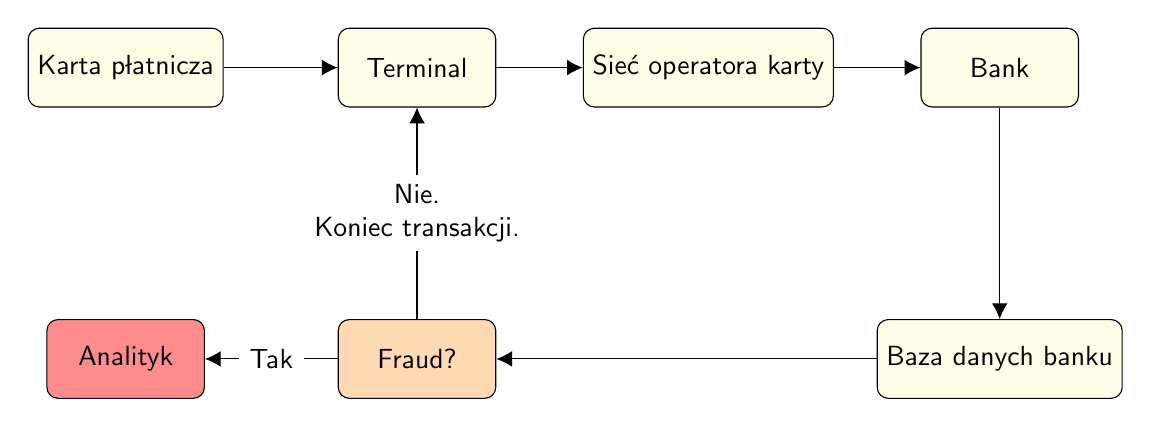
\begin{tikzpicture}[node distance=3.7cm,
			every node/.style={fill=white, font=\sffamily}, align=center]
			% Specification of nodes (position, etc.)
			\node (card)         [base]                        {Karta płatnicza};
			\node (terminal)     [base, right of=card]         {Terminal};
			\node (network)      [base, right of=terminal]     {Sieć operatora karty};
			\node (bank)         [base, right of=network]      {Bank};
			\node (db)           [base, below of=bank]         {Baza danych banku};
			\node (fraud)        [fraud, below of=terminal]    {Fraud?};
			\node (analitic)     [analityk, left of=fraud]     {Analityk};
			
			\draw[->] (card) -- (terminal);
			\draw[->] (terminal) -- (network);
			\draw[->] (network) -- (bank);
			\draw[->] (bank) -- (db);
			\draw[->] (db) -- (fraud);
			\draw[->] (fraud) -- node[text width=0.6cm] {Tak}(analitic);
			\draw[->] (fraud) -- node[text width=4cm] {Nie. \\Koniec transakcji.} (terminal);
		\end{tikzpicture}
	\end{center}

	\caption{Schemat płatności kartą płatniczą. Źródło: Opracowanie własne na podstawie prezentacji A. Bahnsena.}
	\label{fig:credit-card-flow}
\end{figure}

Banki oraz instytucje finansowe w celu przeciwdziałania tym przestępstwom korzystają z~systemów detekcji oszustw. Jest to jeden z elementów całego procesu dokonywania płatności, który jest przedstawiony na rysunku \ref{fig:credit-card-flow} na stronie \pageref{fig:credit-card-flow}. W~momencie przyłożenia karty kredytowej do terminala nawiązywane jest połączenie z operatorem karty (np. Visa, MasterCard), który dalej komunikuje się z bankiem klienta. Następnie w~odpowiednich bazach danych sprawdzane są dostępne środki, a~system detekcji oszustw sprawdza, czy transakcja nie jest podejrzana. W~przypadku wykrycia niezgodności system ją odrzuca i~kieruje sprawę do odpowiedniego analityka. W~przeciwnym razie płatność jest akceptowana i~na~terminalu wyświetla się odpowiedni komunikat.

Do niedawna najbardziej popularnym sposobem do wykrywania oszustw był system oparte na regułach eksperckich.\footnote{Wystąpienie A.Bahnsena podczas Konferencji Analytics 2013. Źródło: \url{https://www.youtube.com/watch?v=YCNkxaVDiA0}} Powstały one na bazie doświadczenia analityków, którzy podczas swojej długoletniej pracy wielokrotnie sprawdzali transakcje pod kątem oszustw i~byli w stanie dostrzec pewne zależności. Przykładami takich reguł mogą być: więcej niż cztery wypłaty z~bankomatu w~ciągu godziny, więcej niż dwie transakcje w~ciągu 5 minut, dwie transakcje w~ciągu 5 minut różnymi formami płatności (karta, internet). W przypadku, gdy rozpatrywana transakcja spełnia chociaż jedną z reguł, to jest ona blokowana i~użytkownik jest informowany o~odrzuceniu transakcji. To podejście jest stosunkowo łatwe do implementacji oraz jest bardzo proste do interpretacji, lecz niestety ma swoje wady. Oszuści wraz z upływem czasu zmieniają swoje sposoby dokonywania oszustw, natomiast systemy złożone z~niemodyfikowalnych reguł nie są w~stanie wykrywać nowych zachowań i dostosowywać się do zmian. Tę niedogodność są w~stanie rozwiązać modele uczenia maszynowego, które tworzą pewnego rodzaju reguły, które nie są bezpośrednio wprowadzane przez użytkownika, lecz automatycznie wykrywane przez algorytmy na podstawie dostarczonych danych historycznych. Wraz z~dynamicznym rozwojem tej dziedziny nauki zaczęły powstawać coraz bardziej wyrafinowane modele, które coraz lepiej radzą sobie z~wykrywaniem takich zależności. Obecnie są one już wykorzystywane w produkcyjnych środowiskach instytucji finansowych i~wspomagają walkę z~przestępcami. Niestety standardowe podejście do modelowania predykcyjnego zakłada równy koszt popełnienia błędu, co nie jest prawdą w tym, jak i~w~wielu innych praktycznych zastosowaniach. Stąd powstała motywacja do rozwoju metod, które biorą pod uwagę tę różnicę.

Wybór tematu pracy był związany z codzienną pracą nad modelami predykcyjnymi wykorzystywanymi do detekcji oszustw w szkodach komunikacyjnych. Zauważony przeze mnie w trakcie prac problem nierównego kosztu pomyłek doprowadził mnie do poszukiwania metod, które będą adekwatne do tego rodzaju wyzwań. W ten sposób trafiłem na prace dr Alejandro Correa Bahnsena, które poruszały to zagadnienie dla modelowania ryzyka kredytowego, prognozy rezygnacji z usług przez klientów, marketingu bezpośredniego oraz detekcji oszustw w transakcjach kartami kredytowymi. Z uwagi na bliską analogię ostatniego przykładu z moim problemem zdecydowałem się na bliższe zapoznanie z tym tematem.

Celem pracy jest opisanie i porównanie standardowych oraz wrażliwych na koszty modeli predykcyjnych w problemie detekcji oszustw na kartach płatniczych. W tym celu zostanie przeprowadzony eksperyment porównujący skuteczność poszczególnych metod. Wykorzystane zostaną modele takie jak regresja logistyczna, drzewo decyzyjne, las losowy oraz algorytm XGBoost wraz z odpowiednimi modyfikacjami oraz metody optymalizacji progu i minimalizacji ryzyka bayesowskiego.

Praca jest zorganizowana w następujący sposób. Rozdział pierwszy jest wstępem teoretycznym, który wprowadza odpowiednie pojęcia i modele z dziedziny statystyki oraz uczenia maszynowego. Rozdział drugi prezentuje opis eksperymentu na danych rzeczywistych wraz z wynikami oraz wnioskami. Ostatnia część podsumowuje całość pracy.

\chapter{Wprowadzenie teoretyczne}

Wprowadzenie teoretyczne zawiera przegląd metod z~dziedziny statystyki oraz uczenia maszynowego, które wykorzystuje się w~zagadnieniach klasyfikacyjnych. W~szczególności zaczniemy od opisania macierzy pomyłek, macierzy kosztu oraz związane z nimi miary skuteczności modeli predykcyjnych, które służą do badania jakości predykcji. Następnie przejdziemy do modeli standardowych, które nie biorą pod uwagi różnych kosztów popełniania błędu klasyfikacyjnego. W~ramach tej grupy opiszemy regresję logistyczną, drzewo decyzyjne, las losowy oraz algorytm XGBoost. Na końcu poruszymy temat modeli wrażliwych na koszt, które dzielimy na dwie podkategorie: trening wrażliwy na koszt (\textit{ang. Cost Sensitive Training}) oraz klasyfikacja wrażliwa na koszt (\textit{ang. Cost Sensitive Classification})\footnote{Źródło:  \url{https://towardsdatascience.com/fraud-detection-with-cost-sensitive-machine-learning-24b8760d35d9}}. Pierwsza z nich zawiera metody, które w trakcie uczenia modelu zwracają uwagę na koszt błędnej klasyfikacji. Są to rozszerzone wersje standardowych modeli, które w~trakcie uczenia się mają zmienioną postać optymalizowanej funkcji. W~tej pracy będziemy omawiać regresję logistyczną wrażliwą na koszt oraz drzewo decyzyjne wrażliwe na koszt. Druga podkategoria składa się z metod, które wykorzystują estymowane prawdopodobieństwo ze~standardowych modeli i~na jego podstawie tworzą dodatkowy model, który bierze pod uwagę koszt niepoprawnej klasyfikacji danego przypadku. Z~tej grupy omówimy optymalizację progu oraz minimalizację ryzyka bayesowskiego.

W pracy będziemy wykorzystywać następujące oznaczenia:
\begin{itemize}
	\item $\es = \{\iks_1, \iks_2, \dots, \iks_N \}$ -- zbiór wszystkich $N$ obserwacji,
	\item $\iks_{i} = \left(x_i^{(1)}, x_i^{(2)}, \dots, x_i^{(j)} \right)$ -- $i$-ty wektor obserwacji składający się z $j$ atrybutów,
	\item $x_i^{(k)}$ -- $k$-ty atrybut $i$-tego wektora obserwacji,
	\item $\ytrue = (y_1, y_2, \dots, y_N)$ - wektor prawdziwych stanów klasyfikacji,
	\item $y_i \in \{0,1\}$ -- prawdziwy stan klasyfikacji dla $i$-tej obserwacji. Wartość $0$ oznacza klasyfikację negatywną, natomiast wartość $1$ oznacza klasyfikację pozytywną.
	\item $p_i \in [0,1]$ -- estymowana wartość prawdopodobieństwa dla $i$-tej obserwacji,
	\item $c_i \in \{0,1\} $ -- przewidywana klasa dla $i$-tej obserwacji. Oznaczenia analogicznie jak dla $y_i$.
\end{itemize}

\section{Miary skuteczności modeli}

\subsection{Macierz pomyłek}

Jedną z metod wykorzystywanych do oceny skuteczności modeli w zadaniach klasyfikacyjnych jest macierz pomyłek. Prawidłowe klasyfikacje zestawiamy z klasami nadanymi przez model, a~następnie sprawdzamy, czy poprawnie zaklasyfikowaliśmy poszczególne obserwacje. W~przypadku klasyfikacji binarnej popełniamy dwa rodzaje błędów, a~wszystkie możliwe wyniki prezentują się w~następujący sposób:
\begin{myitemize}
	& Prawdziwie pozytywny wynik klasyfikacji (TP, z angielskiego \textit{True Positive}) -- obserwacja była pozytywna i zaklasyfikowaliśmy ją jako pozytywną;
	& Fałszywie pozytywny wynik klasyfikacji (FP, z angielskiego \textit{False Positive}) -- obserwacja była negatywna i zaklasyfikowaliśmy ją jako pozytywną. W nomenklaturze statystycznej nazywamy ją również błędem pierwszego rodzaju;
	& Fałszywie negatywny wynik klasyfikacji (FN, z angielskiego \textit{False Negative}) -- obserwacja była pozytywna i zaklasyfikowaliśmy ją jako negatywną. W nomenklaturze statystycznej nazywamy ją również błędem drugiego rodzaju;
	& Prawdziwie negatywny wynik klasyfikacji (TN, z angielskiego \textit{True Negative}) -- obserwacja była negatywna i zaklasyfikowaliśmy ją jako negatywną.
\end{myitemize}
\noindent Liczbę obserwacji należących do poszczególnych kategorii możemy reprezentować tak jak w~tabeli \ref{tab:macierz-pomylek}.
\begin{table}[h]
	\begin{center}
		\begin{tabular}{c|c|c}
			 \multirow{2}{4em}{} & Stan pozytywny & Stan negatywny \\
			                  & $y_i = 1$            & $y_i = 0$ \\
			 \hline
			  Predykcja pozytywna & \multirow{2}{4em}{\centering TP} & \multirow{2}{4em}{\centering FP} \\
			    $c_i = 1$         &                    &                    \\
			 \hline
			 Predykcja negatywna & \multirow{2}{4em}{\centering FN} & \multirow{2}{4em}{\centering TN} \\
			   $c_i = 0$         &                    &                    \\
		\end{tabular}
	\end{center}
	\caption{Macierz pomyłek.}
	\label{tab:macierz-pomylek}
\end{table}

\subsection{Miary skuteczności niewrażliwe na koszt}
Na podstawie macierzy pomyłek (tabela \ref{tab:macierz-pomylek}), którą omawialiśmy w poprzedniej podsekcji, możemy zdefiniować następujące miary skuteczności modeli, które nie biorą pod uwagę kosztu popełnienia błędu. W opisach wykorzystane są elementy pracy D.A. Powersa \cite{evaluation_metrics}.

\subsubsection{Dokładność}
Dokładność (\textit{ang. Accuracy}) mierzy stosunek poprawnie zaklasyfikowanych przypadków do ilości wszystkich obserwacji. Bierze ona pod uwagę zarówno obserwacje pozytywne, jak i negatywne. Z~tego powodu bardzo dobrze radzi sobie w sytuacji, gdy interesują nas obserwacje z obu klas, natomiast dużo gorzej, gdy istotna jest tylko jedna klasa. W~szczególności nie nadaje się ona do problemów z dużą dysproporcją klas, która pojawia się w przypadku detekcji oszustw. Dokładność zdefiniowana jest następującym wzorem
$$ \text{Dokładność} = \frac{TP + TN}{TP + FP + FN + TN} \text{.}$$

\subsubsection{Precyzja}
Precyzja (\textit{ang. Precision}) to stosunek poprawnie zaklasyfikowanych pozytywnych przypadków do wszystkich obserwacji zaklasyfikowanych jako pozytywne. Mierzy ona, jaki procent próbek prawidłowo zaklasyfikowaliśmy jako pozytywne. Warto zauważyć, że nie bierze ona pod uwagę obserwacji negatywnych. Jest ona bardzo często wykorzystywana podczas rozwiązywania większości problemów z~zakresu uczenia maszynowego, ponieważ najczęściej interesuje nas, aby nasze typowania były możliwie najbardziej skuteczne. Z~tego też powodu precyzja jest często nazywana skutecznością klasyfikacji prawdziwie pozytywnych (\textit{ang. True Positive Accuracy}). Zapisana wzorem przyjmuje postać
$$ \text{Precyzja} = \frac{TP}{TP + FP} \text{.}$$

\subsubsection{Czułość}
Czułość (\textit{ang. Recall}) to stosunek prawdziwie pozytywnie zaklasyfikowanych przypadków do wszystkich pozytywnych obserwacji. Innymi słowy, jest to miara, która mówi nam o procencie znalezionych przez model przypadków pozytywnych. Podobnie jak precyzja skupia się jedynie na poprawnie zaklasyfikowanych obserwacjach pozytywnych. Jest ona szczególnie ważna w zastosowaniach medycznych, gdzie naszym głównym celem jest znalezienie wszystkich chorych osób. Używana jest także do wyznaczania krzywej charakterystyki pracy odbiornika (ROC, z angielskiego \textit{Receiver operating characteristic}) opisanej w~sekcji \ref{ROC} na stronie \pageref{ROC}. Czułość jest wyrażona wzorem
$$ \text{Czułość}= \frac{TP}{TP + FN} \text{.}$$

\subsubsection{Swoistość}
Swoistość (\textit{ang. Specificity}) to stosunek prawdziwie negatywnie zaklasyfikowanych przypadków do wszystkich negatywnych obserwacji. Inaczej nazywana też odwrotną czułością, z~uwagi na analogiczną postać do czułości, ponieważ podobnie mierzy ona odsetek znalezionych wszystkich obserwacji, lecz dla negatywnej klasy. Wyraża się następującym wzorem
$$ \text{Swoistość}= \frac{TN}{TN + FP} \text{.}$$

\subsubsection{Ujemna wartość predykcyjna}
Ujemna wartość predykcyjna to stosunek prawdziwie negatywnie zaklasyfikowanych przypadków do wszystkich negatywnie zaklasyfikowanych obserwacji. Nazywana jest również odwrotną precyzją, ponieważ analogicznie do precyzji skupia się na mierzeniu skuteczności klasyfikowania obserwacji negatywnych. Miara ta jest także używana do wyrysowania krzywej ROC (patrz sekcja \ref{ROC} na stronie \pageref{ROC}), a dokładniej wartość $1- \text{ujemna wartość predykcyjna}$, która odpowiada stosunekowi fałszywie pozytywnych klasyfikacji (ang. \textit{false positive ratio}). Dana jest wzorem
$$ \text{Ujemna wartość predykcyjna}= \frac{TN}{TN + FN} \text{.}$$

\subsubsection{Zbalansowana skuteczność} 
Zbalansowana skuteczność (\textit{ang. balanced accuracy}) to średnia arytmetyczna czułości oraz swoistości. W przypadku, gdy klasyfikator działa równie dobrze dla obu klas, to sprowadza się ona do dokładności, natomiast gdy standardowa dokładność jest wysoka tylko z uwagi na niezbalansowaną liczość próbek w klasach, to wartość zbalansowanej skuteczności spada \cite{balanced_accuracy}. Jest ona również ważna, ponieważ maksymalizacja tej miary odpowiada standardowemu szukaniu optymalnego punktu na krzywej ROC (patrz sekcja \ref{ROC} na stronie \pageref{ROC}) wg. metryki taksówkowej. Zadana jest wzorem
$$ \text{Zbalansowana skuteczność}= \frac{\text{Czułość} + \text{Swoistość}}{2} \text{.}$$

\subsubsection{F Score}
$\text{F}_1$ Score to miara łącząca w sobie precyzję oraz czułość za pomocą średniej harmonicznej. Z~uwagi na wykorzystanie tych dwóch wartości nie bierze ona pod uwagę prawidłowo zaklasyfikowanych obserwacji negatywnych. Wykorzystanie średniej harmonicznej powoduje, że kładziemy równy nacisk na obie użyte miary. Standardowy wzór wygląda następująco
$$ \text{F}_1 \text{ Score} = \left(\frac{2}{\text{Precyzja}^{-1} + \text{Czułość}^{-1}}\right) = 2 \cdot \frac{\text{Precyzja} \cdot \text{Czułość}}{\text{Precyzja} + \text{Czułość}} \text{.}$$

W przypadku, gdy interesuje nas bardziej precyzja lub czułość, to definiujemy bardziej ogólną formułę na $\text{F}_{\beta}$ Score:
$$ F_{\beta} = (1 + \beta^2) \cdot \frac{\text{Precyzja} \cdot \text{Czułość}}{(\beta^2 \cdot \text{Czułość}) + \text{Precyzja}} \text{,}$$
gdzie parametr $\beta>0$ odpowiada na pytanie, ile razy bardziej czułość jest ważniejsza niż precyzja. Najczęściej wykorzystuje się parametr $\beta = 2$ lub $\beta = \frac{1}{2}$, który odpowiednio zwiększa nacisk na czułość lub zmniejsza wpływ fałszywie negatywnie zaklasyfikowanych obserwacji, skupiając się bardziej na precyzji.


\subsection{Krzywa charakterystyki pracy odbiornika}
\label{ROC}

Krzywa charakterystyki pracy odbiornika to wykres diagnostyczny modelu predykcyjnego pozwalający na zilustrowanie zdolności klasyfikatora do rozróżniania poszczególnych klas. Składa się ona z wyrysowanym na osi X stosunku fałszywie pozytywnych klasyfikacji na oraz czułości na osi Y \cite{evaluation_metrics}. Miary są narysowane dla różnych wartości progu decyzyjnego, który prawdopodobieństwa zwracane przez model zamienia na decyzje binarne. Perfekcyjny klasyfikator jest w stanie osiągnąć lewy górny róg wykresu, czyli posiadać precyzję na poziomie 100\% oraz stosunek fałszywie pozytywnych klasyfikacji na poziomie 0\%. Analogicznie najgorszy klasyfikator jest w stanie osiągnąć prawy dolny róg wykresu. Model losowy będzie prostą z punktu $(0,0)$ do punktu $(1,1)$. 

Przykładowy wykres znajduje się na rysunku \ref{fig:roc_example} na stronie \pageref{fig:roc_example}. Kolorem czerwonym oznaczony jest najgorszy możliwy klasyfikator, zielonym perfekcyjny, niebieskim losowy, natomiast żółtym przykładowy.

\begin{figure}[h]
	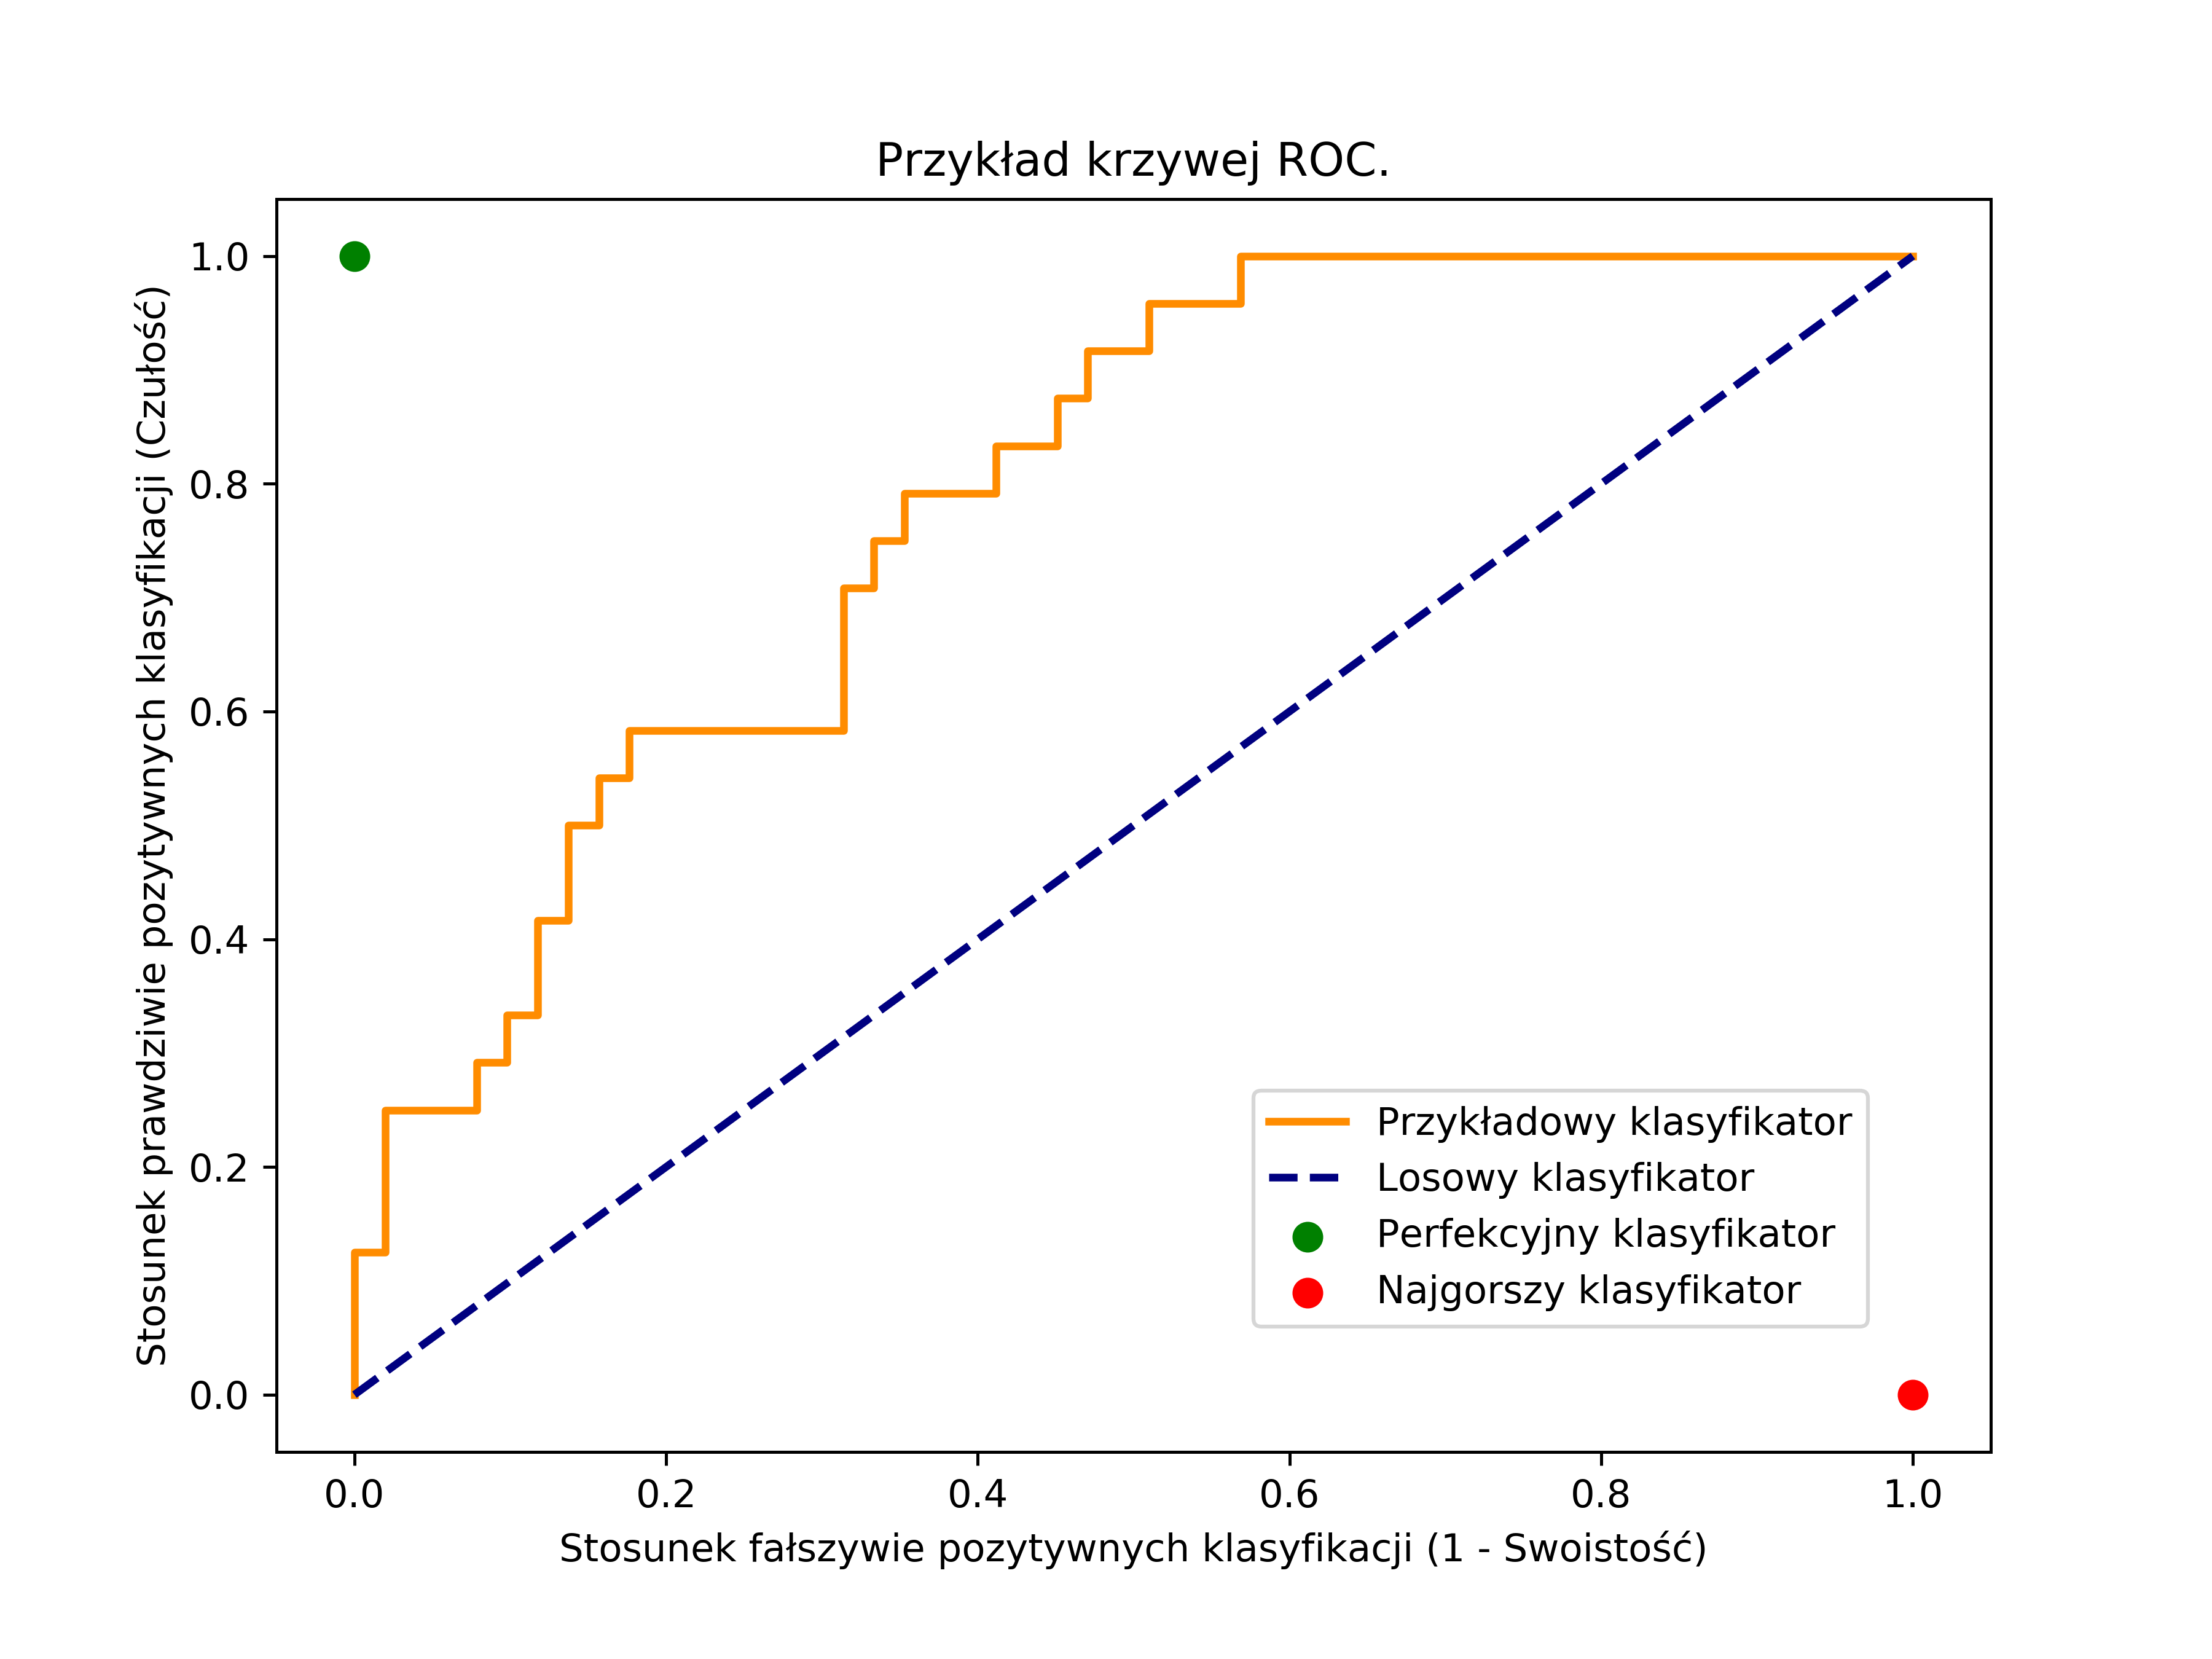
\includegraphics[width=\linewidth]{images/roc_example.png}
	\caption{Przykładowy wykres charakterystyki pracy odbiornika. Na poziomej osi przedstawiony jest stosunek fałszywie pozytywnych klasyfikacji, natomiast na pionowej czułość. Kolorem czerwonym, zielonym, niebieskim oraz żółtym jest odpowiednio oznaczony najgorszy, najlepszy, losowy oraz przykładowy klasyfikator. Źródło: Opracowanie własne.}
	\label{fig:roc_example}
\end{figure}

\subsection{Macierz kosztu}
\label{sec:macierz-kosztu}
W celu wprowadzenia potrzebnych miar skuteczności wrażliwych na koszt potrzebujemy najpierw zdefiniować macierz kosztu $C$ \cite{CSCCFD, CS-Learning}. Ma ona postać analogiczną do macierzy pomyłek, lecz zamiast ilość obserwacji w odpowiednich komórkach wpisujemy koszt pomyłki dla $i$-tej obserwacji. Warto zaznaczyć, że koszt niekoniecznie musi być kwota pieniężną, lecz także możemy rozważać ilość poświęconego czasu, bądź inną dowolną mierzalną jednostkę. W szczególności dla przypadku klasyfikacji binarnej wyróżniamy cztery możliwe wartości:
\begin{myitemize}
	& \underscoretext{C}{TP}{i} -- koszt prawdziwie pozytywnego zaklasyfikowania $i$-tej obserwacji,
	& \underscoretext{C}{FP}{i} -- koszt fałszywie pozytywnego zaklasyfikowania $i$-tej obserwacji,
	& \underscoretext{C}{FN}{i} -- koszt fałszywie negatywnego zaklasyfikowania $i$-tej obserwacji,
	& \underscoretext{C}{TN}{i} -- koszt prawdziwie negatywnego zaklasyfikowania $i$-tej obserwacji.
\end{myitemize}

W zależności od praktycznego zastosowania wartości w macierzy kosztu przyjmują różne wielkości. Poniżej przedstawiamy kilka intuicji na podstawie macierzy kosztu zdefiniowanych dla różnych eksperymentów w~pracy A. Bahnsena \cite{alej2015ensemble}.
\begin{itemize}
	\item W przypadku, gdy predykcja klasy pozytywnej wiąże się z podjęciem jakiejś akcji, np. sprawdzenie transakcji kartą kredytową, wysłanie oferty reklamowej, to koszt pozytywnej predykcji jest dodatni, to znaczy \underscoretext{C}{TP}{i}, \underscoretext{C}{FP}{i} $>0$. Ponadto najczęściej te koszty są równe i przyjmują stałą wartość dla wszystkich przypadków, to znaczy \underscoretext{C}{TP}{i}~$=$~\underscoretext{C}{FP}{i}~$= \text{const.}$, ponieważ podejmowana zawsze jest ta sama akcja dla wszystkich obserwacji. Dodatkowo koszt pozytywnego zaklasyfikowania dla każdej obserwacji negatywnej jest zerowy, to znaczy \underscoretext{C}{TN}{i} $=0$, ponieważ słusznie nie została podjęta żadna akcja. Zatem ostatecznie jedyną wartością, która różni się między przypadkami, jest koszt fałszywie negatywnej klasyfikacji i on również jest większy od zera.
	\item W przypadku, gdy predykcja dokonywana jest przez zautomatyzowany system, to koszt prawidłowej klasyfikacji jest równy zero, to znaczy \underscoretext{C}{TP}{i}~$=$~\underscoretext{C}{TN}{i}~$=0$, ponieważ maszynie nie musimy płacić pensji, która obsługuje daną sprawę. Natomiast koszty pomyłek są różne i zazwyczaj różnią się między obserwacjami. Biorąc jako przykład ryzyko kredytowe, możemy zauważyć, że koszty mogą być zarówno dodatnie, jak i ujemne. W tym konkretnym przypadku, gdy stwierdzimy, że dana osoba spłaci kredyt, natomiast w rzeczywistości nie zrobi tego, to będziemy stratni pewną sumę pieniędzy, co da nam dodatni koszt. Z drugiej strony, gdy uznamy, że dana osoba nie spłaci kredytu, a w rzeczywistości wywiązałaby się z zobowiązań, to utracimy pewien zarobek, zatem koszt będzie negatywny.
\end{itemize}

Koncepcyjnie koszt popełnienia błędu dla każdej obserwacji powinien być większy niż koszt poprawnej klasyfikacji, to znaczy
$$ \text{C}_{\text{FP}_{\text{i}}} >\text{C}_{\text{TP}_{\text{i}}} \text{ i } \text{C}_{\text{FN}_{\text{i}}} > \text{C}_{\text{TN}_{\text{i}}} \quad \forall_{i \in \{1, 2, \dots, N\}} \text{.}$$
Natomiast jak możemy zauważyć na podstawie wyżej opisanych intuicji, w praktycznych zastosowaniach jest to bardzo często nierealistyczne założenie.
% TODO: Opisać warunki na koszty, gdyby wszystkie były stałe.
Przykład takiej macierzy kosztu znajduje się w tabeli \ref{tab:macierz-kosztu}.
\begin{table}[h]
	\begin{center}
		\begin{tabular}{c|c|c}
			\multirow{2}{4em}{} & Stan pozytywny & Stan negatywny \\
			& $y_i = 1$            & $y_i = 0$ \\
			\hline
			Predykcja pozytywna & \multirow{2}{4em}{\centering \underscoretext{C}{TP}{i}} & \multirow{2}{4em}{\centering \underscoretext{C}{FP}{i}} \\
			$c_i = 1$         &                    &                    \\
			\hline
			Predykcja negatywna & \multirow{2}{4em}{\centering \underscoretext{C}{FN}{i}} & \multirow{2}{4em}{\centering \underscoretext{C}{TN}{i}} \\
			$c_i = 0$         &                    &                    \\
		\end{tabular}
	\end{center}
	\caption{Macierz kosztu.}
	\label{tab:macierz-kosztu}
\end{table}

\subsection{Miary skuteczności modeli wrażliwych na koszt}
Motywacją do powstania miar skuteczności wrażliwych na koszt jest potrzeba ewaluacji modeli, która miarodajnie odda złożoność rozwiązywanego problemu \cite{EDCSLR}. Przykładowo w~przypadku detekcji oszustw będzie w stanie odpowiedzieć na pytanie dotyczące zaoszczędzonej kwoty dzięki modelowi predykcyjnemu. Kolejny powodem jest fakt, że podstawowe metryki nie uwzględniają różnicy w kosztach pomyłki dla fałszywie pozytywnych oraz fałszywie negatywnych klasyfikacji, traktując oba błędy jednakowo. Ponadto warto zauważyć, że omawiane problemy wymagają uwzględnienia nie tylko różnych kosztów per rodzaj pomyłki, ale także per konkretna obserwacja. Bazując na wprowadzonej w sekcji \ref{sec:macierz-kosztu} macierzy kosztu $C$, zdefiniujemy kilka miar.

\subsubsection{Koszt}
Rozpoczniemy od matematycznego wprowadzenia kosztu, który wyznacza jaką wartość powinniśmy wziąć z macierzy kosztu $C_i$ dla $i$-tej obserwacji mając daną predykcję oraz prawdziwą wartość klasyfikacji.
$$ \text{Koszt}(y_i, c_i, C_i) = y_i \left(c_i C_{TP_i} + (1-c_i)C_{FN_i}\right) + (1-y_i)\left(c_i C_{FP_i} + (1-c_i)C_{TN_i}\right) \text{,}$$
gdzie $C_{TP_{i}}\text{,} C_{FP_{i}}\text{,} C_{FN_{i}}\text{,} C_{TN_{i}}$ to odpowiednie wartości z macierzy kosztu $C_i$.

\subsubsection{Koszt całkowity}
Koszt całkowity (TC, z angielskiego \textit{ang. Total Cost}) to suma kosztów poniesionych dla danego zestawy predykcji $\boldsymbol{c}$, który zostały wygenerowany przez pewien model predykcyjny. Definiowany jest wzorem
\begin{equation}
	\label{koszt-calkowity}
	\text{TC}(\ytrue, \boldsymbol{c}, \boldsymbol{C}) = \sum_{i=1}^{N}\text{Koszt}(y_i, c_i, C_i) \text{,}
\end{equation} 
gdzie:
\begin{itemize}
	\item $\boldsymbol{c} = (c_1, c_2, \dots, c_N) $ - wektor przewidywanych klas,
	\item $\boldsymbol{C} = (C_1, C_2, \dots, C_N) $ - wektor macierzy kosztu.
\end{itemize}

\subsubsection{Oszczędności}
Oszczędności (\textit{ang. Savings}) to miara, którą intuicyjnie możemy rozumieć jako procentową wartość, o~ile testowany model jest lepszy od naiwnego klasyfikatora. Przy czym naiwnym klasyfikatorem nazywamy model, który zwraca same predykcje pozytywne lub same predykcje negatywne, w~zależności od tego, co bardziej się opłaca dla danego zestawu danych.
\begin{equation}
	\label{oszczednosci}
	\text{Oszczędności}(\ytrue, \boldsymbol{c}, \boldsymbol{C}) = \frac{\text{Koszt bazowy}(\ytrue, \boldsymbol{C}) - \text{TC}(\ytrue, \boldsymbol{c}, \boldsymbol{C})}{\text{Koszt bazowy}(\ytrue, \boldsymbol{C})} \text{,}
\end{equation}
gdzie:
\begin{itemize}
	\item $ \text{Koszt bazowy}(\ytrue, \boldsymbol{C}) = \min\{\text{TC}(\ytrue, \boldsymbol{c}_0, \boldsymbol{C}), \text{TC}(\ytrue, \boldsymbol{c}_1, \boldsymbol{C})\}$ - koszt poniesiony w przypadku używania naiwnego klasyfikatora,
	\item $\boldsymbol{c}_0 = (0, 0, \dots, 0)$ - wektor $N$-elementowy predykcji równych $0$,
	\item $\boldsymbol{c}_1 = (1, 1, \dots, 1)$ - wektor $N$-elementowy predykcji równych $1$.
\end{itemize}{}
% TODO: Analiza wartości minimalnych oraz maksymalnych Kosztu całkowitego oraz Oszczędności. 

\section{Standardowe modele}

\subsection{Regresja logistyczna}
\label{reg-log}
Regresja logistyczna jest bardzo ważnym modelem statystycznym, którego celem jest modelowanie prawdopodobieństwa, że zmienna losowa $Y$ przyjmie wartość $0$ lub $1$, na~podstawie danych empirycznych. Rozważmy następującą definicję modelu regresji logistycznej parametryzowaną wektorem współczynników $\theta = (\theta_1, \theta_2, \dots, \theta_n)$ daną w~następujący sposób
\begin{equation}
	\htx = \frac{1}{1+e^{-\iks_{i}\theta^T}} = P(Y = 1|X = \iks_{i};\theta) \text{.}
\end{equation} 
Jednocześnie zauważmy, że
$$ P(Y = 0|X = \iks_{i};\theta) = 1 - P(Y = 1|X = \iks_{i};\theta) = 1 - \htx $$
oraz korzystając z faktu, że $y_i \in \{0,1\}$, możemy zapisać 
$$ P(Y = y_i|\iks_{i};\theta) = \htx^{y_i}(1-\htx)^{(1-y_i)} \text{.}$$
Następnie zakładając, że wszystkie obserwacje są niezależne i~pochodzą z~rozkładu Bernoulliego, wyznaczamy funkcję największej wiarygodności, aby wyestymować parametry~$\theta$.
$$ L(\theta | \es) = \prod_{i=1}^N P(Y = y_i | X = \iks_{i}; \theta) = \prod_{i=1}^N \htx^{y_i}(1-\htx)^{(1-y_i)}$$
W celu znalezienia maksimum funkcji wiarygodności logarytmujemy funkcję $L(\theta | \es)$ i~otrzymujemy funkcję straty $J(\theta)$
$$ J(\theta) = \log L(\theta | \es)  = \frac{1}{N} \sum_{i=1}^N J_i(\theta)\text{,}$$
gdzie $J_i(\theta)$ nazywana jest entropią krzyżową i przyjmuje postać
\begin{equation}
	\label{c-e}
	J_i(\theta) = -y_i\log(h_{\theta}(\boldsymbol{x_i})) - (1-y_i)\log(1 - h_{\theta}(\boldsymbol{x_i})) \text{.}
\end{equation}
Niestety nie jest możliwe znalezienie bezpośredniego wzoru na współczynniki, które maksymalizują funkcję wiarygodności, zatem wykorzystuje się w tym celu algorytmy optymalizacji numerycznej, np. metodę Newtona.

\begin{figure}[h]
	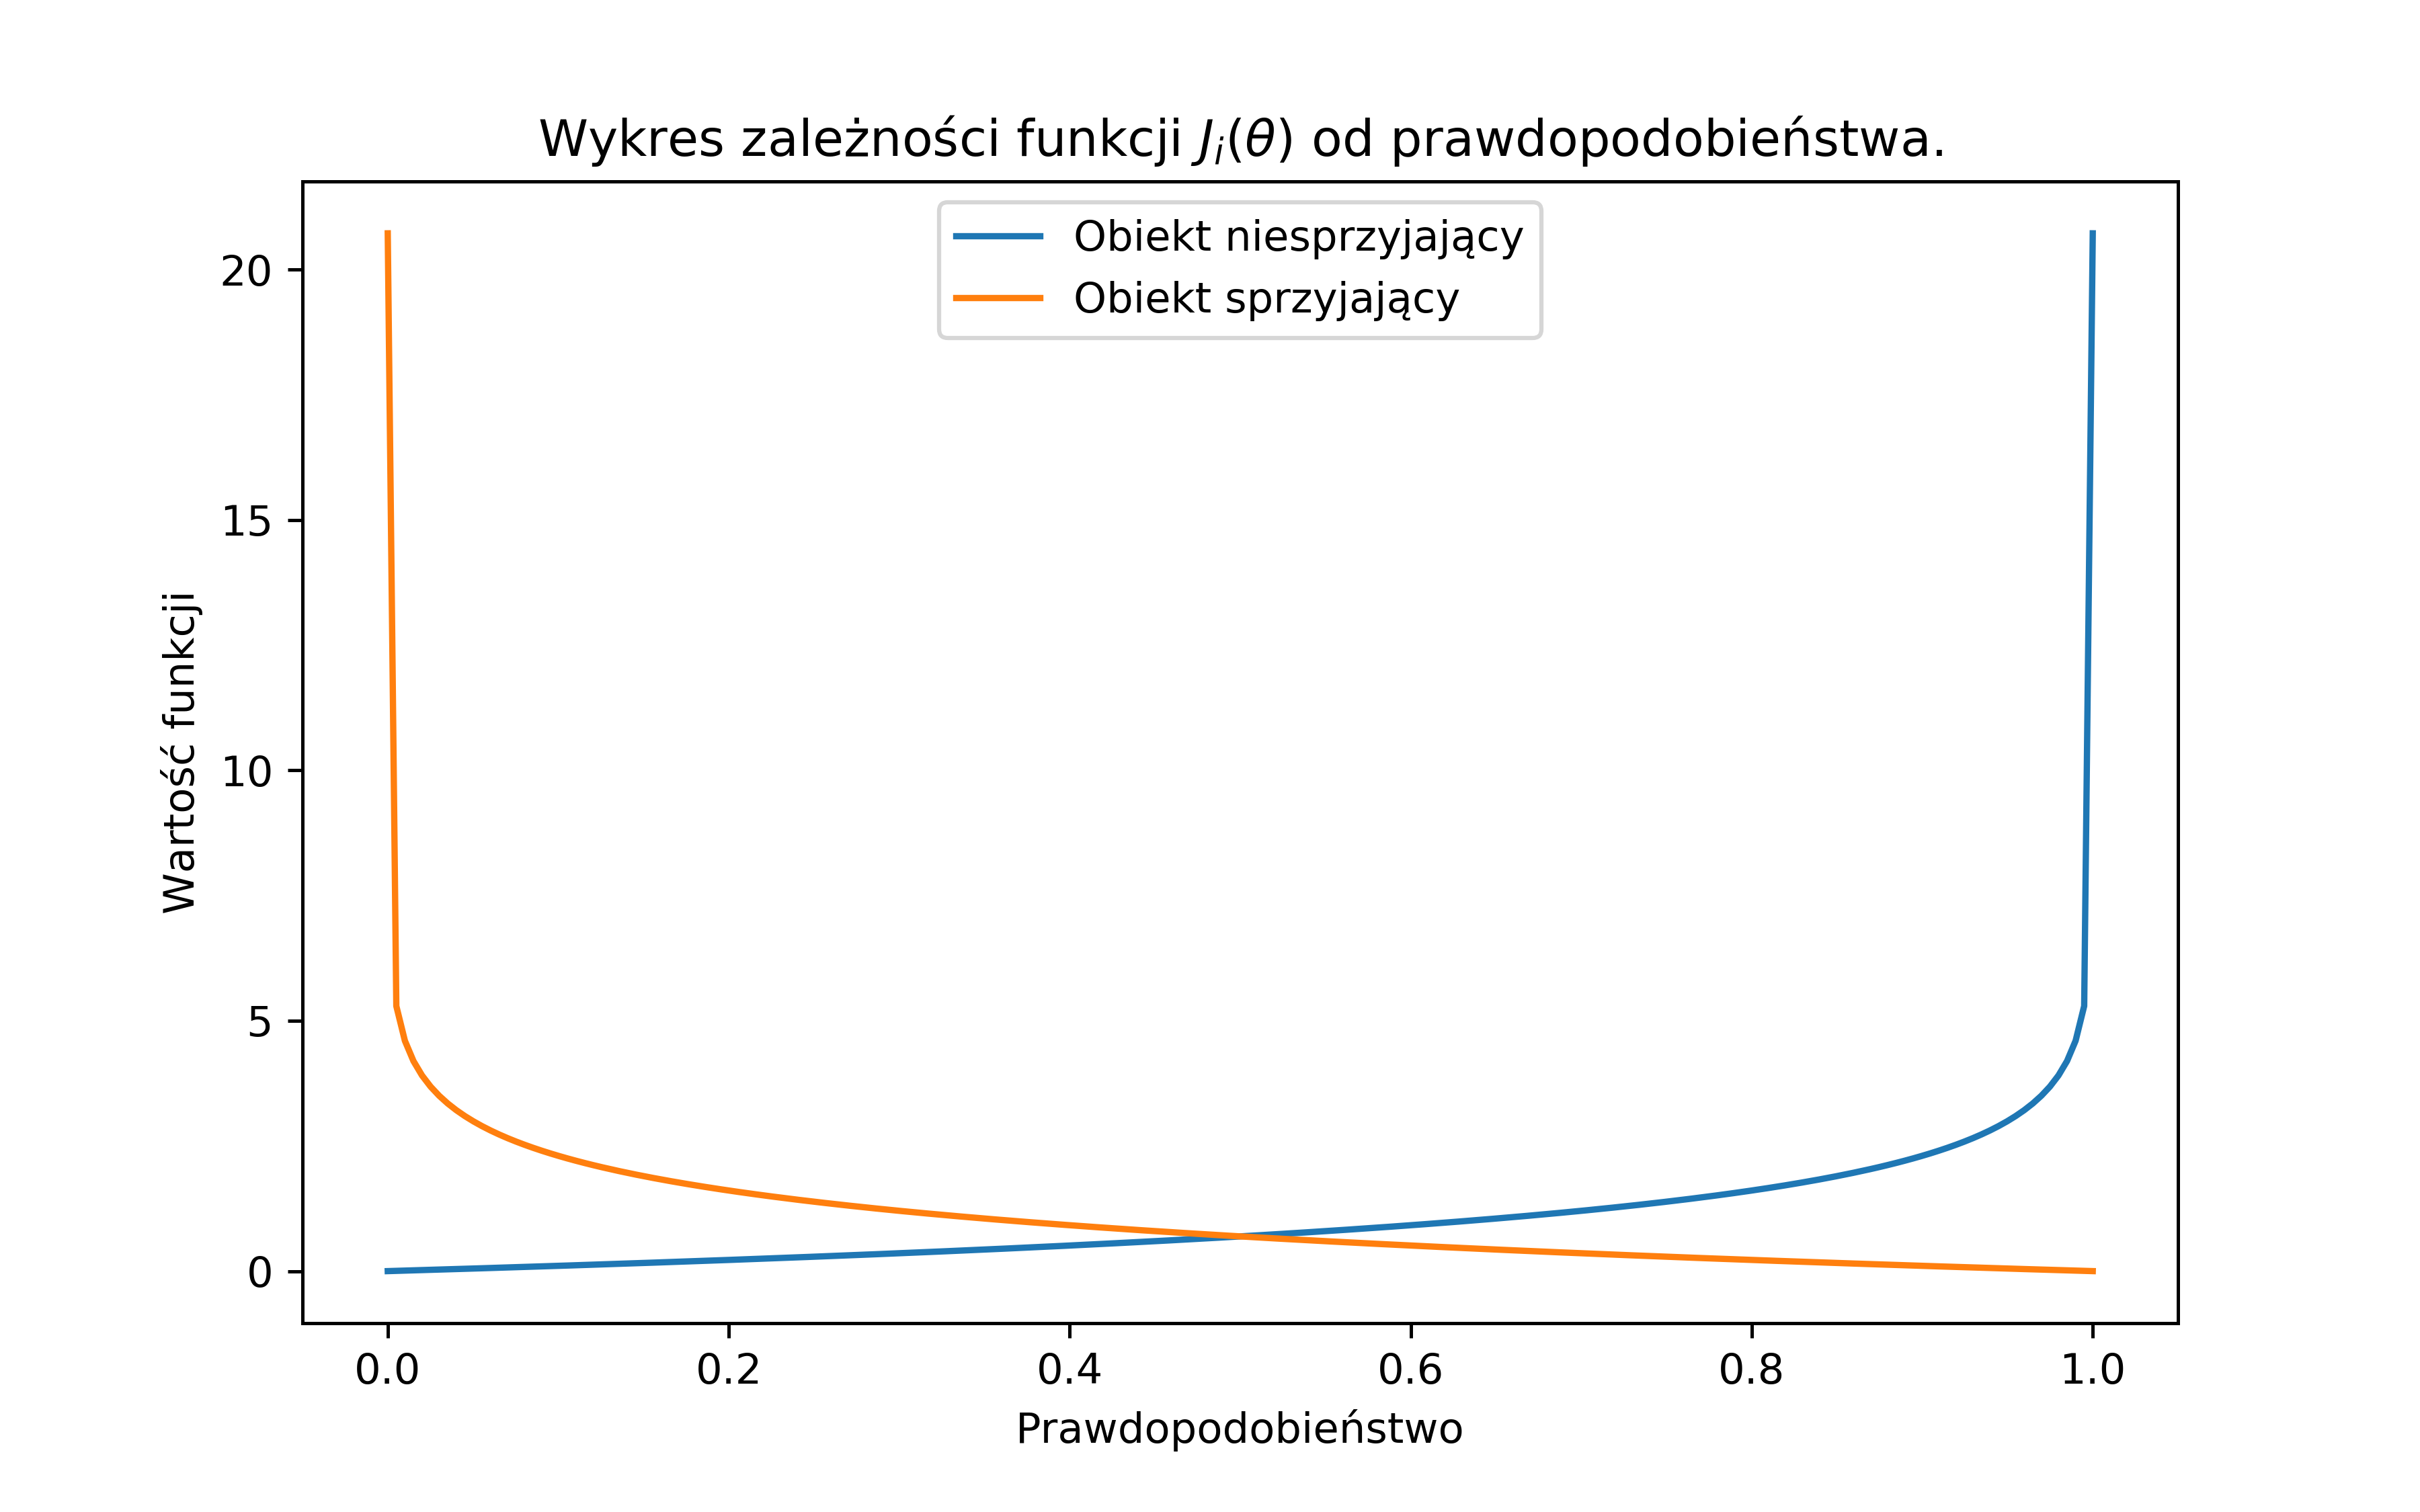
\includegraphics[width=\linewidth]{images/cross_entropy.png}
	\caption{Wykres zależności funkcji entropii krzyżowej od prawdopodobieństwa predykcji danej obserwacji. Kolor niebieski przedstawia wykres dla próbki o prawdziwej klasie pozytywnej, natomiast kolor pomarańczowy dla negatywnej. Źródło: Opracowanie własne.}
	\label{fig:cross-entropy-plot}
\end{figure}

Zauważmy, że maksymalizowana funkcja wiarygodności jest sumą wartości entropii krzyżowej dla poszczególnych obserwacji. W celu lepszego zrozumienia całości przyjrzymy się bliżej własnościom funkcji $J_i(\theta)$.

Wykres \ref{fig:cross-entropy-plot} ze strony \pageref{fig:cross-entropy-plot} przedstawia przyjmowane wartości funkcji $J_i(\theta)$ w zależności od estymowanego prawdopodobieństwa $\htx$. Kolorem niebieskim jest wyznaczony przebieg funkcji dla klasy negatywnej, a pomarańczowym dla pozytywnej. Możemy zauważyć, że funkcja jest symetryczna względem wartości prawdopodobieństwa $0.5$ dla obu klas. Oznacza to, że ten klasyfikator przykłada taką samą wagę dla obu rodzajów błędów. Ponadto koszt klasyfikacji dla pojedynczej obserwacji przyjmuje w przybliżeniu następujące wartości:
$$
J_i(\theta) \approx \left\{
\begin{array}{rl}
0, &\mbox{jeżeli $y_i \approx \htx$}, \\
\infty, &\mbox{jeżeli $y_i \approx (1 - \htx)$}.
\end{array}{}
\right.
$$
To znaczy, że w przypadku prawidłowego zaklasyfikowania danej obserwacji funkcja przyjmuje wartość bliską zeru, natomiast w przypadku pomyłki nieskończoności. Stąd możemy wywnioskować, że koszty popełnienia bądź niepopełnienia błędu są następujące:
$$ C_{TP_i} = C_{TN_i} \approx 0 \text{,}$$
$$ C_{FP_i} = C_{FN_i} \approx \infty \text{.}$$
Jest to wynik, który nie oddaje charakteru nierówności kosztu popełniania różnych błędów, stąd powstaje motywacja, aby zmodyfikować podaną funkcję i stworzyć regresję logistyczną, która będzie w stanie modyfikować koszty poszczególnych klasyfikacji.

\subsection{Drzewo decyzyjne}
\label{drzewo}
Drzewo decyzyjne to nieparametryczny model uczenia nadzorowanego, który jest wykorzystywany do regresji oraz klasyfikacji. Jego celem jest nauczenie się na podstawie dostępnych danych prostych reguł decyzyjnych. Do jego największych zalet należy prostota interpretacji otrzymanych wyników oraz mała ilość potrzebnych przygotowań danych.

Wyróżniamy trzy rodzaje algorytmów, które są odpowiedzialne za proces uczenia drzew. Poniżej krótki opis każdego z nich.
\begin{itemize}
	\item ID3 (Iterative Dichotomiser 3) -- algorytm pozwala na tworzenie drzew decyzyjnych, które w poszczególnych węzłach mogą mieć więcej niż dwa podziały. Działa jedynie dla zmiennych kategorycznych. Drzewo rośnie do maksymalnego rozmiaru, a następnie jest przycinane;
	\item C4.5 -- następca ID3, który znosi restrykcję używania tylko kategorycznych atrybutów poprzez dyskretyzację zmiennych ciągłych. Następnie nauczone drzewo zamieniane jest w zestaw reguł, które są szeregowane względem poprawy skuteczności. Przycinanie w tym wypadku polega na usuwanie reguł, które nie poprawiają wyniku modelu;
	\item CART (z angielskiego \textit{Classification and Regression Tree}) -- bardzo podobny algorytm do C4.5, który umożliwia tworzenie drzew regresyjnych (w poprzednich algorytmach mamy do czynienia jedynie z zadaniami klasyfikacyjnymi) oraz nie tworzy zestawu reguł. Konstruuje on binarne drzewa, które do podziału używa atrybutu oraz progu odcięcia, który maksymalizuje przyrost informacji.
\end{itemize}
Warto zaznaczyć, że implementacja w bibliotece \textit{sklearn} w Pythonie wykorzystuje zmodyfikowaną wersję algorytmu CART, który nie obsługuje zmiennych kategorycznych. Poniżej prezentujemy teorię matematyczną stojącą za implementacją tego algorytmu \cite{sklearn_api}.

Niech $\ku$ będzie zbiorem obserwacji dla danego węzła $m$. Ponadto niech podział będzie reprezentowany przez parę $\theta = (j, t_m)$, gdzie $j$ to $j$-ty atrybut wektora $\iks_i$, a $t_m$ to warunek podziału danych na podzbiory $\ku_l$ oraz $\ku_r$, gdzie
$$ \ku_l (\theta) = \{ \iks_i : \iks_i \in \ku \land x^{j}_i \leq t_m \} \text{,} $$
$$ \ku_r (\theta) = \ku \setminus \ku_l(\theta) \text{.} $$
Czystość danego węzła jest wyznaczana w następujący sposób
$$ G(\ku, \theta) = \frac{|\ku^l|}{|\ku|} I(\ku_l (\theta)) + \frac{|\ku^r|}{|\ku|} I(\ku_r (\theta)) \text{,}$$
gdzie $I(\cdot)$ może być dowolną miarą zanieczyszczenia. Ostatecznie w~danym węźle wybierany jest ten podział, który minimalizuje funkcję czystości
$$ \theta^* = \argmin_\theta G(\ku, \theta) \text{.}$$
Dalej następuje podział na podzbiory $\ku_l (\theta^*)$ i $\ku_r (\theta^*)$ i algorytm działa rekurencyjnie, aż do osiągnięcia maksymalnej głębokości. Ostatnie podziały, które pozostały na końcu drzewa, nazywamy liśćmi i w momencie predykcji klasyfikują one daną próbkę lub zwracają odpowiednie prawdopodobieństwo.
W zależności od implementacji oraz preferencji użytkownika po zakończeniu działania algorytmu wykorzystuje się przycinanie drzew. Jest to metoda, która w ogólności polega na usuwanie nadmiarowych węzłów, które mogą powodować zbyt dokładne dopasowanie do danych. 

W~zależności od rodzaju problemu wykorzystujemy różne miary zanieczyszczenia. Dla zadań klasyfikacyjnych są to
\begin{itemize}
	\item Misclassification: $I_m(\ku) = 1 - \max(p, 1 - p)$,
	\item Entropy: $I_e(\ku) = -p \log_2 p - (1 - p) \log_2(1 - p)$,
	\item Gini: $I_g(\ku) = 2p(1 - p)$,
\end{itemize}{}
a dla zadań regresyjnych
\begin{itemize}
	\item $ \displaystyle I_{mse}(\ku) = \frac{1}{|\ku|} \sum_{i \in \ku} (y_i - q)^2$,
	\item $ \displaystyle I_{mae}(\ku) = \frac{1}{|\ku|} \sum_{i \in \ku} |y_i - q|$,
\end{itemize}
gdzie:
$$ p = \frac{| \{ \iks_i : \iks_i \in \ku \land y_i = 1 \}|}{|\ku|} \text{,} $$
$$ q = \frac{\sum_{i \in \ku} y_i}{|\ku|} \text{.} $$

\subsection{Las losowy}
Las losowy oraz algorytm XGBoost są przedstawicielami szerokiej klasy modeli typu \textit{ensemble}. Głównym celem tej metodologii jest wprowadzenie losowych perturbacji do zbioru treningowego w celu utworzenia różnych klasyfikatorów bazowych, których wspólne predykcje będą lepsze niż każdego z modeli bazowych osobno. Istnieją ponadto trzy główne powody, dlaczego te metody działają znacznie lepiej niż pojedyncze modele.
\begin{itemize}
	\item Statystyczny -- w przypadku, gdy mamy do czynienia z małym zbiorem danych, istnieje możliwość stworzenia kilku bardzo dobryh klasyfikatorów, które na zbiorze treningowym mają taką samą skuteczność. W przypadku dodatkowego zbioru testowego istnieje szansa wybrania nieoptymalnego;
	\item Obliczeniowy -- większość algorytmów polega na optymalizacji numerycznej, która może zatrzymać się w minimum lokalnym. Dzięki zastosowaniu kilku modeli uzyskujemy szansę przeszukania większej części przestrzeni parametrów modeli;
	\item Reprezentacyjny -- często funkcja $f$ reprezentująca prawdziwy model jest bardzo skomplikowana i niemożliwe jest przedstawienie jej za pomocą jednego modelu. Wykorzystując złożenie kilku modeli bazowych, mamy szansę lepiej przybliżać prawdziwą funkcję $f$.
\end{itemize}

W celu utworzenia $T$ klasyfikatorów bazowych należy ze zbioru treningowego $\es$ wybrać $S_j$ dla $j=1,2,\dots,T$ losowych podzbiorów obserwacji, które wykorzystamy do uczenia. W tym celu wykorzystuje się następujące procedury losowania.

\begin{itemize}
	\item Wklejanie (\textit{Pasting}) -- Polega na niezależnym losowaniu $K < N$ próbek ze zbioru $\es$ bez powtórzeń. Najczęściej wykorzystywana jest na bardzo dużych zbiorów danych, gdzie zasoby obliczeniowe są ograniczone i nie jest możliwe wczytanie wszystkich danych do pamięci komputera. Ponadto dzięki możliwości wykorzystania obliczeń równoległych skraca się czas tworzenia całego modelu. Próbki mogą być losowane z rozkładu jednostajnego bądź wykorzystując metody biorące pod uwagę ważność poszczególnych obserwacji. \cite{Pasting}
	\item Workowanie (\textit{ang. Bagging}) -- Polega na niezależnym losowaniu $K \leq N$ próbek ze zbioru $\es$ z powtórzeniami. Najczęściej jest wykorzystywany w przypadku małych zbiorów danych, kiedy chcemy wykorzystać maksymalnie dużą ilość obserwacji, lecz także wprowadzić losowość do kolejnych klasyfikatorów bazowych.
	\item Losowe podprzestrzenie (\textit{ang. Random Subspaces}) -- Metoda polegająca na wybraniu do każdego klasyfikatora bazowego wszystkich obserwacji, lecz losuje się tylko część atrybutów opisujące dane. Głównym celem tego zabiegu jest poprawa skuteczności poprzez zwiększenie różnorodności klasyfikatorów bazowych. \cite{Random_Subspace}
	\item Losowe łaty (\textit{ang. Random Patches}) -- Procedura łącząca metodę wklejania z losowymi podprzestrzeniami. Jej celem jest połączenie zalet obu metod i ostatecznie poprawienie skuteczności modelu z~jednoczesną optymalizacją wykorzystywanego czasu oraz pamięci. \cite{Random_Patches}
\end{itemize}
Warto zauważyć, że mimo tego, że powyższe metody były oryginalnie tworzone z myślą o wykorzystaniu drzewa decyzyjnego jako klasyfikatora bazowego, to nic nie stoi na przeszkodzie wykorzystać inny model. Ten fakt został między innymi wykorzystany w~pracy A.Bahnsena \cite{alej2015ensemble}, gdzie wykorzystując omawiane w sekcji \ref{csdt} drzewa decyzyjne wrażliwe na koszt, stworzono lasy losowe wrażliwe na koszt.

Procedura tworzenia lasu losowego jest podzielona na dwie fazy \cite{Random_Forest}. Pierwsza z nich wykorzystuje workowanie do wygenerowania odpowiednich próbek dla klasyfikatorów bazowych. Następnie trenujemy zmodyfikowane drzewa decyzyjne, które na etapie tworzenia każdego kolejnego węzła w drzewie losują podzbiór zmiennych do wyboru podziału. Finalnie podczas predykcji każdy model dokonuje klasyfikacji i ostatecznym wynikiem modelu jest większość głosów. Nie jest to jedyna możliwość agregowania wyników, przykładowo wykorzystywana w bibliotece \textit{sklearn} w Python implementacja uśrednia wyniki prawdopodobieństwa z każdego klasyfikatora \cite{sklearn_api}.

\subsection{XGBoost}
Algorytm XGBoost (lub z~angielskiego \textit{Extreme Gradient Boosting})to model, który w iteracyjny sposób tworzy kolejne drzewa decyzyjne typu CART opisywane w~sekcji \ref{drzewo} \cite{xgboost}. Jest to podobnie jak w przypadku lasu losowego złożenie wielu klasyfikatorów bazowych, stąd możemy zapisać predykcję $i$-tej obserwacji jako
$$ \hat{y_i} = \sum_{k=1}^K f_k(\iks_i) \text{,} \quad f_k \in \ef \text{,} $$
gdzie $K$ oznacza liczbę drzew decyzyjnych, $f$ funkcje z przestrzeni $\ef$ wszystkich możliwych drzew CART.
W ogólności proces trenowania modeli w uczeniu maszynowym polega na znalezieniu najlepszych parametrów $\theta$, które najlepiej pasują do danych treningowych ze zbioru $\es$ i ich prawdziwych wartości $\ytrue$. W celu dokonania tego procesu definiujemy funkcję celu (\textit{ang. objective}), którą w ogólnej postaci możemy zapisać jako
$$ \text{Obj}(\theta) = J(\theta) + \Omega(\theta) \text{,}$$
gdzie $J(\theta)$ to funkcja straty, a $\Omega$ to wyraz odpowiadający za regularyzację, która nakłada odpowiednie kary na współczynniki modelu, aby zapobiec zbytniemu dopasowaniu do danych. Za funkcję straty najczęściej przyjmujemy w przypadku zadań regresyjnych błąd średnio kwadratowy
$$ J(\theta) = \sum_{i=1}^{N} (y_i - \bar{y})^2 $$
lub w przypadku zadań klasyfikacyjnych entropię krzyżową daną równaniem \ref{c-e}.

Przechodząc na bardziej jawne wzory, funkcja celu w kroku iteracji $t$ przyjmuje postać
\begin{equation}
	\label{Obj}
	\text{Obj}^{(t)}(\theta) = \sum_{i=1}^{N} l(y_i, \yht{t}) + \sum_{k=1}^{K} \Omega(f_k) \text{,}
\end{equation}
gdzie $l(y_i, \yht{t})$ to w innej formie zapisana funkcja straty $J(\theta)$, a $\yht{t}$ oznacza wartość predykcji w kroku $t$.
W przypadku tego algorytmu wykorzystamy trening addytywny, który polega na iteracyjnym poprawianiu nieprawidłowych klasyfikacji z poprzednich modeli poprzez odpowiednie przydzielanie wag próbkom w kolejnych fazach. Zatem dalej mamy
$$ \yht{0} = 0 $$
$$ \yht{1} = f_1(x_i)  = \yht{0} + f_1(x_i) $$
$$ \yht{2} = f_1(x_i) + f_2(x_i) = \yht{1} + f_2(x_i) $$
$$ ... $$
$$ \yht{t} = \sum_{k=1}^{t} f_k(x_i) = \yht{t-1} + f_t(x_i) $$
Korzystając z powyższych wzorów oraz \ref{Obj} otrzymujemy następujące wyrażenie
$$ \text{Obj}^{(t)}(\theta) = \sum_{i=1}^{n} l(y_i, \yht{t-1} + f_t(x_i)) + \Omega(f_t) + \text{const. .}$$
Korzystając z rozwinięcia szeregu Taylora dla funkcji straty, otrzymujemy ogólny wzór:
$$ \text{Obj}^{(t)}(\theta) = \sum_{i=1}^{n} \left[ l(y_i, \yht{t-1}) + g_i f_t(x_i) + \frac{1}{2} h_i f_t^2(x_i) \right] + \Omega(f_t) + \text{const. ,} $$
gdzie 
$$ g_i = \partial_{\yht{t-1}} l(y_i, \yht{t-1}) \text{,} $$
$$ h_i = \partial^2_{\yht{t-1}} l(y_i, \yht{t-1}) \text{.}$$
Następnie po redukcji stałych, które są nieistotne z punktu widzenia optymalizacji, otrzymujemy
$$ \sum_{i=1}^{n} [g_i f_t(x_i) + \frac{1}{2} h_i f_t(x_i)] + \Omega(f_t) \text{.}$$
Zauważmy, że nigdzie bezpośrednio nie korzystaliśmy z postaci funkcji straty, zatem w ten sposób jesteśmy w stanie zbudować model optymalizujący dowolną dwukrotnie różniczkowalną funkcję ciągłą. Taka uniwersalność powoduje, że algorytm ten znajduje zastosowanie w wielu zadniach z zakresu uczenia maszynowego, jak i innych problemów optymalizacyjnych.

\section{Klasyfikacja wrażliwa na koszt}
Metody klasyfikacji wrażliwej na koszt (\textit{ang. Cost Dependent Classification})  są przykładem pierwszego rodzaju modeli wrażliwych na koszt. W przypadku tych metod trening odbywa się dopiero po etapie stworzenia modelu zwracającego prawdopodobieństwa i informacja o koszcie jest uwzględniana dopiero w tej fazie modelowania. Cały proces jest przedstawiony na Rysunku \ref{cdc} na stronie \pageref{cdc}. Górna część diagramu przedstawia standardowy proces uczenia modelu predykcyjnego, natomiast dolna część reprezentuje schemat dokonywania predykcji, w którym najpierw estymujemy prawdopodobieństwa dla zbioru testowego, a następnie wykorzystując te wartości oraz koszt klasyfikacji dokonujemy ostatecznej decyzji, czy dana obserwacja jest pozytywna, czy negatywna. Warto wspomnieć, że w celu dokonania kolejnego treningu modelu potrzebujemy podzbioru danych, który nie był wykorzystywany do uczenia podstawowego modelu. Najczęściej taki zbiór nazywamy walidacyjnym.
\begin{figure}
	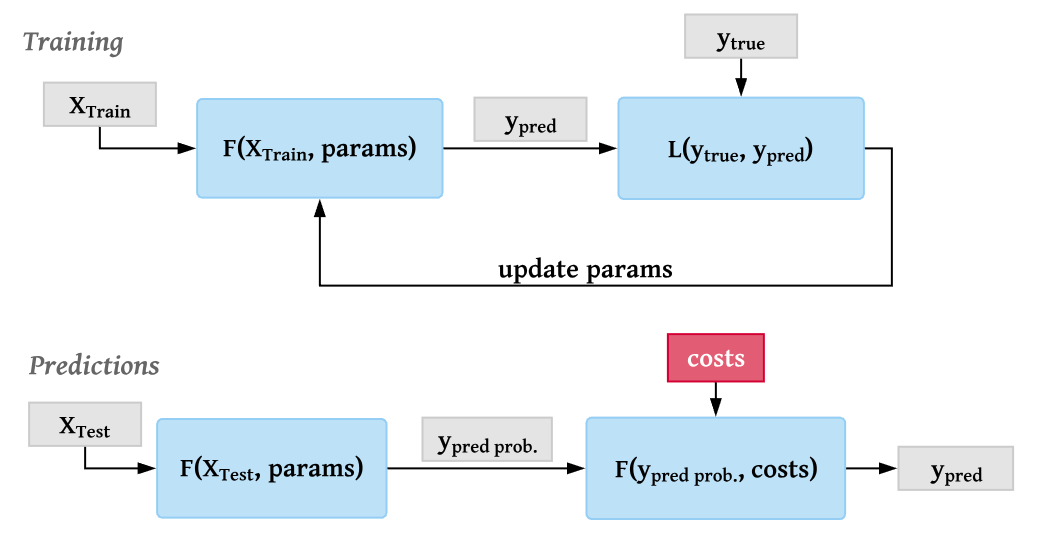
\includegraphics[width=\linewidth]{images/cost_sensitive_classification.png}
	\caption{Schemat przedstawiający proces uczenia klasyfikatora wrażliwego na koszt. Źródło: \url{https://towardsdatascience.com/fraud-detection-with-cost-sensitive-machine-learning-24b8760d35d9}}
	\label{cdc}
\end{figure}
\subsection{Optymalizacja progu}
Metoda optymalizacji progu (TO z angielskiego \textit{threshold optimization}) jest popularną metodą wyznaczania odpowiedniego progu prawdopodobieństwa, powyżej którego wszystkie obserwacje oznaczamy jako pozytywnie zaklasyfikowane, a poniżej negatywnie. Może być ona wykorzystywana nie tylko do problemów wrażliwych na koszt, lecz do dowolnie zdefiniowanego zagadnienia, w którym potrzebne są zero-jedynkowe predykcje. Jej sformułowanie wygląda następująco
$$ \argmin_{t \in [0,1]} f(\ytrue, \boldsymbol{y}_{\text{decision}}) \text{,} $$
gdzie 
\begin{itemize}
	\item $f(\cdot, \cdot) $ - funkcja miary skuteczności modelu, która jako argumenty przyjmuje wektor prawdziwych wartości klasyfikacji oraz wektor binarnych predykcji, np. dokładność,
	\item $\boldsymbol{y}_{\text{decision}} = (p_i > t)_{i=1}^n $ - wektor binarnych klasyfikacji modelu,
	\item $ \text{t} $ - wartość progu decyzyjnego.
\end{itemize}{}
W naszym przypadku funkcją $f$ będzie funkcja oszczędności (\ref{oszczednosci}). Innymi słowy, będziemy szukać takiego progu decyzyjnego, który zmaksymalizuje wartość oszczędności.

\subsection{Minimalizacja ryzyka bayesowskiego}
Minimalizacja ryzyka bayesowskiego (BMR z angielskiego \textit{Bayesian Minimum Risk}) to model decyzyjny, którego celem jest zmierzenie oraz porównanie wartości prawdopodobieństw wystąpienia pewnych zdarzeń i kosztów związanych z podjęciem określonych decyzji  \cite{CSCCFD}. Polega na przypisaniu odpowiedniej wartości reprezentującej ryzyko zaklasyfikowania danej obserwacji jako pozytywnej lub negatywnej, które definiujemy w następujący sposób
$$ R(p_1|\iks_{i}) = L(p_1|y_1)P(y_1|\iks_{i}) + L(p_1|y_0)P(y_0|\iks_{i}) \text{,}$$
$$ R(p_0|\iks_{i}) = L(p_0|y_0)P(y_0|\iks_{i}) + L(p_0|y_1)P(y_1|\iks_{i}) \text{,}$$
gdzie
\begin{itemize}
	\item $P(p_1|\iks_{i})$, $P(p_0|\iks_{i})$ - oznaczają estymowane przez model prawdopodobieństwa zaklasyfikowania obserwacji jako odpowiednio pozytywna oraz negatywna klasa i~$P(p_0|\iks_{i}) = 1 - P(p_1|\iks_{i})$,
	\item $L(p_{i}|y_{j})$ oraz $i,j \in \{0, 1\}$ - funkcja kosztu, która określa stratę, którą poniesiemy w zależności od wyniku poprawności klasyfikacji.
\end{itemize}{}
Decyzja dotycząca danej obserwacji jest opisana następującą nierównością
$$ R(p_1|\iks_{i}) \leq R(p_0|\iks_{i})$$
i oznacza ona, że klasyfikujemy dany przykład jako pozytywny, jeżeli ryzyko takiej decyzji jest mniejsze niż zaklasyfikowania danej obserwacji jako negatywną. 
Po przeprowadzaniu odpowiednich przekształceń algebraicznych otrzymujemy następujący wzór na klasyfikację przykładu jako pozytywny:
$$ P(p_1|\iks_{i}) \ge \frac{L(p_1|y_0) - L(p_0|y_0)}{L(p_0|y_1) - L(p_1|y_1) - L(p_0|y_0) + L(p_1|y_0)} \text{.}$$
W przypadku gdy za funkcję kosztu przyjmiemy odpowiednie wartości z macierzy kosztu, to otrzymamy następujący próg decyzyjny
$$ p \ge \frac{C_{FP_i} - C_{TN_i}}{C_{FN_i} - C_{TP_i} - C_{TN_i} + C_{FP_i}} \text{.}$$

\section{Trening wrażliwy na koszt}
Drugą podgrupą metod wrażliwych na koszt jest trening wrażliwy na koszt (\textit{ang. Cost Sensitive Trainig}). Są to metody, które już na etapie treningu modelu biorą pod uwagę koszt związany z klasyfikacją danej obserwacji. Schemat uczenia modelu jest przedstawiony na wykresie \ref{cst} na stronie \pageref{cst}. Model jako wejście otrzymuje zbiór danych treningowych, następnie dokonuje predykcji i na bazie prawdziwych odpowiedzi oraz kosztów wyznaczana jest skuteczność modelu. W następnej kolejności aktualizowane są wagi, a cały proces jest iteracyjnie powtarzany aż do momentu osiągnięcia zadanego kryterium stopu.
\begin{figure}[h]
	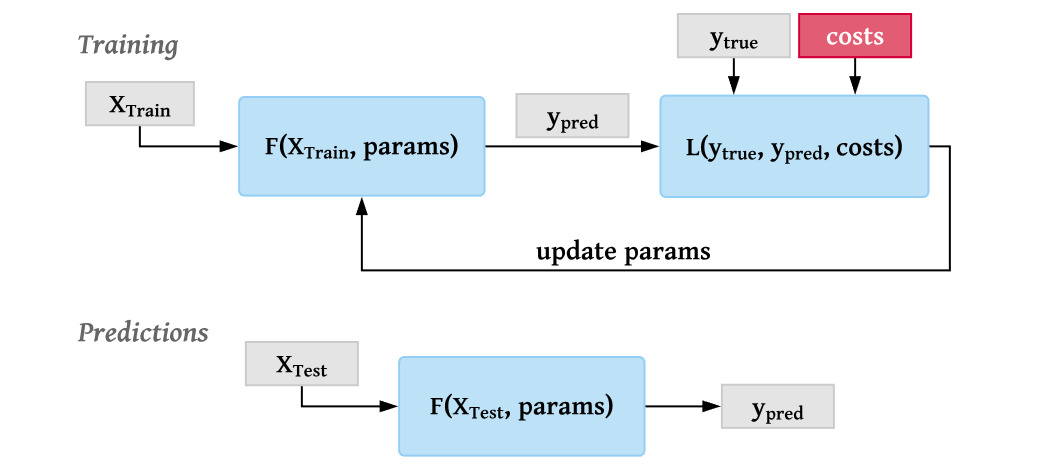
\includegraphics[width=\linewidth]{images/cost_sensitive_training.png}
	\caption{Schemat przedstawiający proces uczenia modelu wrażliwego na koszt. Źródło: \url{https://towardsdatascience.com/fraud-detection-with-cost-sensitive-machine-learning-24b8760d35d9}}
	\label{cst}
\end{figure}	

\subsection{Regresja logistyczna wrażliwa na koszt}
Pierwszy modelem, który stosunkowo łatwo przystosować do bycia wrażliwym na koszt jest regresja logistyczna. Kontynuując rozważania z podrozdziału \ref{reg-log}, chcemy, aby funkcja straty przyjmowała następujące wartości, które odpowiadają wartościom z~macierzy kosztu:
$$
J^c_i(\theta)=\left\{
\begin{array}{rl}
C_{TP_i}, &\mbox{jeżeli $y_i = 1$ i $\htx \approx 1$}, \\
C_{TN_i}, &\mbox{jeżeli $y_i = 0$ i $\htx \approx 0$}, \\
C_{FP_i}, &\mbox{jeżeli $y_i = 0$ i $\htx \approx 1$}, \\
C_{FN_i}, &\mbox{jeżeli $y_i = 1$ i $\htx \approx 0$}.
\end{array}
\right.
$$
W rezultacie funkcją, która zachowuje się w następujący sposób, jest
\begin{talign*}
	J^c_i(\theta) &= y_i \Big( \htx C_{TP_i} + (1 - \htx)C_{FN_i} \Big) + (1-y_i) \Big( \htx C_{FP_i} + (1 - \htx)C_{TN_i} \Big) \text{.}
\end{talign*}

\begin{figure}[h]
	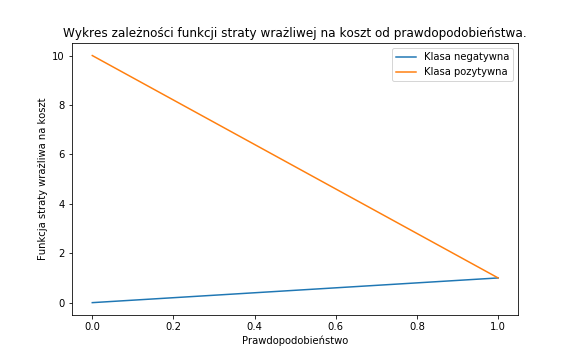
\includegraphics[width=\linewidth]{images/cost_sensitive_ce.png}
	\caption{Wykres zależności wrażliwej na koszt funkcji straty od prawdopodobieństwa predykcji danej obserwacji. Kolor niebieski przedstawia wykres dla próbki o prawdziwej klasie pozytywnej, natomiast kolor pomarańczowy dla negatywnej. Wykres dla przykładowych wartości: $C_{\text{TP}} = 1 \text{, } C_{\text{FN}} = 10 \text{, } C_{\text{FP}} = 1 \text{, } C_{\text{TN}} = 0$. Źródło: Opracowanie własne.}
	\label{fig:cost-sensitive-loss-function}
\end{figure}

Wykres funkcji $J^c_i(\theta)$ jest przedstawiony na wykresie \ref{fig:cost-sensitive-loss-function} na stronie \pageref{fig:cost-sensitive-loss-function}. Kolorem niebieskim zaznaczona jest predykcja dla klasy negatywnej, a pomarańczowym dla pozytywnej. Możemy zauważyć pożądaną przez nas asymetrię popełniania błędów oraz dokładne wartości, jakie funkcja przyjmuje podczas odpowiednich rodzajów błędów.

Ostatecznie funkcją, którą będziemy minimalizować, jest 
$$ J^c(\theta) = \frac{1}{N} \sum_{i=1}^{N} J^c_i(\theta) \text{.} $$
Następnie podobnie jak w przypadku standardowej regresji logistycznej wykorzystujemy odpowiedni algorytm optymalizujący, który znajdzie odpowiednie współczynniki modelu.

\subsection{Drzewo decyzyjne wrażliwe na koszt}
\label{csdt}
Analogicznie jak w przypadku regresji logistycznej w celu wprowadzenia kosztu do treningu drzewa decyzyjnego musimy uzależnić proces powstawania modelu od kosztu danej próbki. Naturalnym miejscem dla drzewa decyzyjnego jest moment podziału danego węzła. Do tej pory wszystkie miary zanieczyszczenia skupiały się na możliwe najlepszym rozróżnieniu próbek w kontekście minimalizacji ilości błędów klasyfikacji. Zamiast tego, w przypadku metody wrażliwej na koszt, naszym celem jest minimalizacja kosztu. W tym celu definiujemy następującą miarę zanieczyszczenia
$$ I_c(\ku) = \text{Koszt bazowy}(\ytrue^{\ku}, \boldsymbol{C}^{\ku}) \text{,}$$
gdzie górny indeks $\ku$ oznacza odpowiedni podzbiór obserwacji, które wybieramy do wektora $\ytrue$ oraz $\boldsymbol{C}$. Intuicja stojąca za takim sformułowaniem jest następująca. Klasyfikujemy wszystkie przypadki w rozważanym podziale jako pozytywne, następnie jako negatywne i sprawdzamy, która z decyzji miała mniejszy sumaryczny koszt. W momencie predykcji ostateczny werdykt, który może być tylko binarny, zależy od tego, która klasyfikacja minimalizuje sumaryczny koszt na liściu.

\chapter{Eksperyment}
W celu porównania zaprezentowanych metod przeprowadzimy eksperyment, którego celem będzie zbadanie ich skuteczności na przykładowym zbiorze danych. 


\section{Dane}
Do eksperymentu zostanie wykorzystany zbiór danych Credit Card Fraud Detection\footnote{Źródło: \url{https://www.kaggle.com/mlg-ulb/creditcardfraud}}, który był stworzony w celu badań naukowych grupy Worldline and the Machine Learning Group\footnote{\url{http://mlg.ulb.ac.be}} z~Université Libre de Bruxelles. Zawiera on 284,807 transakcji w tym zaledwie 492 oszustw. Tabela składa się z 30 kolumn, w tym 28 z nich to zanonimizowane zmienne numeryczne, które były wcześniej poddane transformacji PCA (\textit{ang. Principal Component Analysis}), a dodatkowo mamy informacje dot. czasu transakcji oraz kwoty. Ponadto wśród danych nie ma brakujących wartości. Podczas modelowania pominiemy zmienną czasową, ponieważ sama w sobie nie zawiera ona istotnej informacji, a tworzenie znaczących zmiennych nie jest istotą przeprowadzanego eksperymentu. 

Mimo tego, że dane zostały poddane anonimizacji, to na podstawie artykułu A. Bahnsena możemy domyślać się, z jakimi zmiennymi mieliśmy do czynienia przed transformacjami \cite{CSCCFD}. Podczas procesu dokonywania transakcji standardowo zbierane są: 
\begin{itemize}
	\item data dokonania transakcji, 
	\item numer konta,
	\item numer karty,
	\item typ transakcji (płatność internetowa, płatność stacjonarna, wypłata z bankomatu),
	\item kwota, 
	\item ID beneficjenta transakcji,
	\item grupa beneficjenta transakcji (przykładowo linie lotnicze, hotel, wypożyczalnia samochodów itp.), 
	\item kraj dokonania transakcji,
	\item kraj zamieszkania właściciela karty,
	\item typ karty (przykładowo VISA, MasterCard itp.),
	\item wiek klienta, 
 	\item płeć klienta,
	\item bank klienta,
	\item historyczna informacja czy dana transakcja była oszustwem.
\end{itemize}
Na podstawie wymienionych informacji tworzy się agregaty czasowe bazujące na historii, których celem jest zebranie informacji dotyczących nawyków zakupowych danego klienta\footnote{Wystąpienie A.Bahnsena podczas Konferencji Analytics 2013. Źródło: \url{https://www.youtube.com/watch?v=YCNkxaVDiA0}}. Stworzenie takiej zmiennej polega na zgrupowaniu transakcji w ciągu pewnego odcinka czasowego najpierw według id klienta lub karty kredytowej, dalej przez typ transakcji, beneficjenta transakcji, kategorię beneficjenta lub kraj, kończąc agregacją poprzez zsumowanie ilości bądź wartości tych płatności. Przykładowymi zmiennymi, które powstają w tym procesie, są: ilość transakcji dla tego samego klienta w ciągu ostatnich 6 godzin, średnia wartość transakcji w sklepach spożywczych dla danej karty kredytowej z ostatniego tygodnia. 

% TODO
Informacja, która jest najbardziej istotna z punktu widzenia naszego modelowania, to rozkład oraz charakterystyka zmiennej dot. kwoty transakcji. Na Rysunku znajduje się wykres rozkładu ... 

Warto zauważyć, że najpopularniejszymi wartościami transakcji są: 

Na podstawie wiedzy dotyczącej modelowania detekcji fraudów z artykułu A. Bahnsena \cite{alej2015ensemble} oraz przeprowadzonej wcześniej analizy definiujemy w Tabeli \ref{tab:macierz-kosztu-eksperyment} macierz kosztu dla tego eksperymentu. Wartość $C_a = 1$ to stały koszt administracyjny podjęcia sprawy przez analityka, który sprawdza, czy dana obserwacja jest faktycznie oszustwem, niezależnie od tego, jaki był jego ostateczny werdykt, $\text{Amt}_i$ to wartość transakcji, jaką utracimy w~przypadku niewskazanie fałszywej transakcji jako oszustwa, natomiast zerowa wartość kosztu dla normalnej obserwacji, która była prawidłowo wskazana, pochodzi z~braku konieczności podjęcia inwestygacji oraz strat z tego wynikających.

\begin{table}[h]
	\begin{center}
		\begin{tabular}{c|c|c}
			\multirow{2}{4em}{} & Stan pozytywny & Stan negatywny \\
			& $y_i = 1$            & $y_i = 0$ \\
			\hline
			Predykcja pozytywna & \multirow{2}{8em}{\centering \underscoretext{C}{TP}{i} $ = \text{C}_{\text{a}} = 1$} & \multirow{2}{8em}{\centering \underscoretext{C}{FP}{i} $ = \text{C}_{\text{a}} = 1$} \\
			$c_i = 1$         &                    &                    \\
			\hline
			Predykcja negatywna & \multirow{2}{8em}{\centering \underscoretext{C}{FN}{i} $ = \text{Amt}_{\text{i}}$} & \multirow{2}{8em}{\centering \underscoretext{C}{TN}{i} $ = 0$} \\
			$c_i = 0$         &                    &                    \\
		\end{tabular}
	\end{center}
	\caption{Macierz kosztu eksperymentu.}
	\label{tab:macierz-kosztu-eksperyment}
\end{table}

\section{Opis eksperymentu}
Inspiracja do eksperymentu pochodzi z pracy A.Bahnsena dotyczącej porównania metod wrażliwych na koszt dla pięciu rzeczywistych zbiorów danych pochodzących z czterech dziedzin zastosowań: detekcja oszustw na kartach kredytowych, prognoza rezygnacji, ryzyko kredytowe oraz marketing bezpośredni \cite{alej2015ensemble}. Naszym celem będzie porównanie standardowych metod oraz metod wrażliwych na koszt na innym zbiorze danych. W~tym celu wykorzystamy regresję logistyczną, drzewo decyzyjne, las losowy, XGBoost, drzewo decyzyjne wrażliwe na koszt, a także standardowe modele rozszerzymy metodą optymalizacji progu (TO) oraz minimalizacji ryzyka bayesowskiego (BMR). Dodatkowym rozszerzeniem w stosunku do oryginalnego eksperymentu będzie użycie algorytmu XGBoost, który w wielu przypadkach uzyskuje znacznie lepsze wyniki od reszty modeli uczenia maszynowego, a także spowodowanie, aby brał pod uwagę koszty pomyłek poprzez użycie klasyfikacji wrażliwej na koszt.

W celu przeprowadzenia eksperymentu pięćdziesięciokrotnie dzielimy zbiór danych w~proporcjach 50:17:33 na odpowiednio zbiór treningowy, walidacyjny oraz testowy. Losowanie nowych podziałów zbioru ma na celu zmniejszenie ryzyka, że wynik zależy od wylosowanej próbki. Ponadto wykorzystano tę technikę zamiast standardowej warstwowej walidacji krzyżowej (\textit{ang. Stratified Cross Validation}) z uwagi na chęć uniknięcia zbyt małej próbki testowej w przypadku walidacji krzyżowej z dużą ilością podziałów. Następnie uczymy wszystkie modele standardowe oraz modele z grupy treningu wrażliwego na koszt na zbiorze treningowym. Dla modelu XGBoost wykorzystujemy zbiór walidacyjny do procesu wczesnego zatrzymywania (\textit{ang. Early stopping}), natomiast dla modeli BMR oraz TO korzystamy z tego zbioru jako zbiór treningowy. Następnie dla wszystkich modeli dokonujemy predykcje na zbiorze testowym i mierzymy skuteczność typowań, wykorzystując miarę skuteczności oszczędności oraz $F_1$ Score. 
Ostatecznie wyniki z wszystkich pięćdziesięciu prób uśredniamy oraz obliczamy wartość odchylenia standardowego.

Do implementacji skryptów został wykorzystany język programowania Python wraz z~bibliotekami \textit{costcla}, \textit{sklearn}, \textit{pandas}, \textit{numpy}, \textit{matplotlib} oraz język programowania bash.

\section{Wyniki}

Wyniki eksperymentu dla miary skuteczności oszczędności są zaprezentowane na wykresie \ref{fig:results-savings} na stronie \pageref{fig:results-savings}. Szare, niebieskie oraz czerwone słupki oznaczają dla pierwszych czterych modeli: regresji logistycznej (LogisticRegression), drzewa decyzyjnego (DecisionTree), lasu losowego (RandomForest) oraz XGBoosta, odpowiednio model standardowy, model po optymalziacji progu oraz model wykorzystujący minimalizację ryzyka bayesowskiego. Dla modelu drzewa decyzyjnego wrażliwego na koszt (CS Decision Tree) mamy jedynie szary słupek, ponieważ model ten sam w sobie jest już wrażliwy na koszt i nie potrzebuje dodatkowych modyfikacji. 

Możemy zauważyć, że wśród standardowych modeli oraz drzewa decyzyjnego wrażliwego na koszt najmniejszy wynik oszczędności uzyskała regresja logistyczna a najlepszy las losowy, XGBoost oraz drzewo decyzyjne wrażliwe na koszt. Ponadto wrażliwa na koszt wersja drzewa decyzyjnego również przynosi lepsze rezultaty. W~przypadku, gdy weźmiemy pod uwagę rozszerzone wersje modeli standardowych o klasyfikację wrażliwą na koszt, to zdecydowanie najlepszym modelem staje się XGBoost w~połączeniu z~minimalizacją ryzyka bayesowskiego. Warto zauważyć, że w~przypadku optymalizacji progu wartość oszczędności jest co najmniej równa bądź większa niż wynik uzyskany przez standardowy model. Dla minimalizacji ryzyka bayesowskiego zachodzi podobna sytuacja, gdzie w~każdym przypadku wyniki są lepsze. Ponadto średnia wartość oszczędności tego modelu w~obrębie każdego z modeli standardowych jest najwyższa. Podsumowując, w~przypadku tego eksperymentu, gdyby najważniejsza byłaby dla nas wartość oszczędności po wprowadzeniu modelu predykcyjnego, to najlepszym wyborem byłby algorytm XGBoost z dodatkowym modelem minimalizacji ryzyka bayesowskiego. Dodatkowo w~każdym z~przypadków model wrażliwy na koszt poprawia wynik oszczędności. Spójrzmy jednak, jak zmienia się ogólna moc predykcyjna modelu.

\begin{figure}[h]
	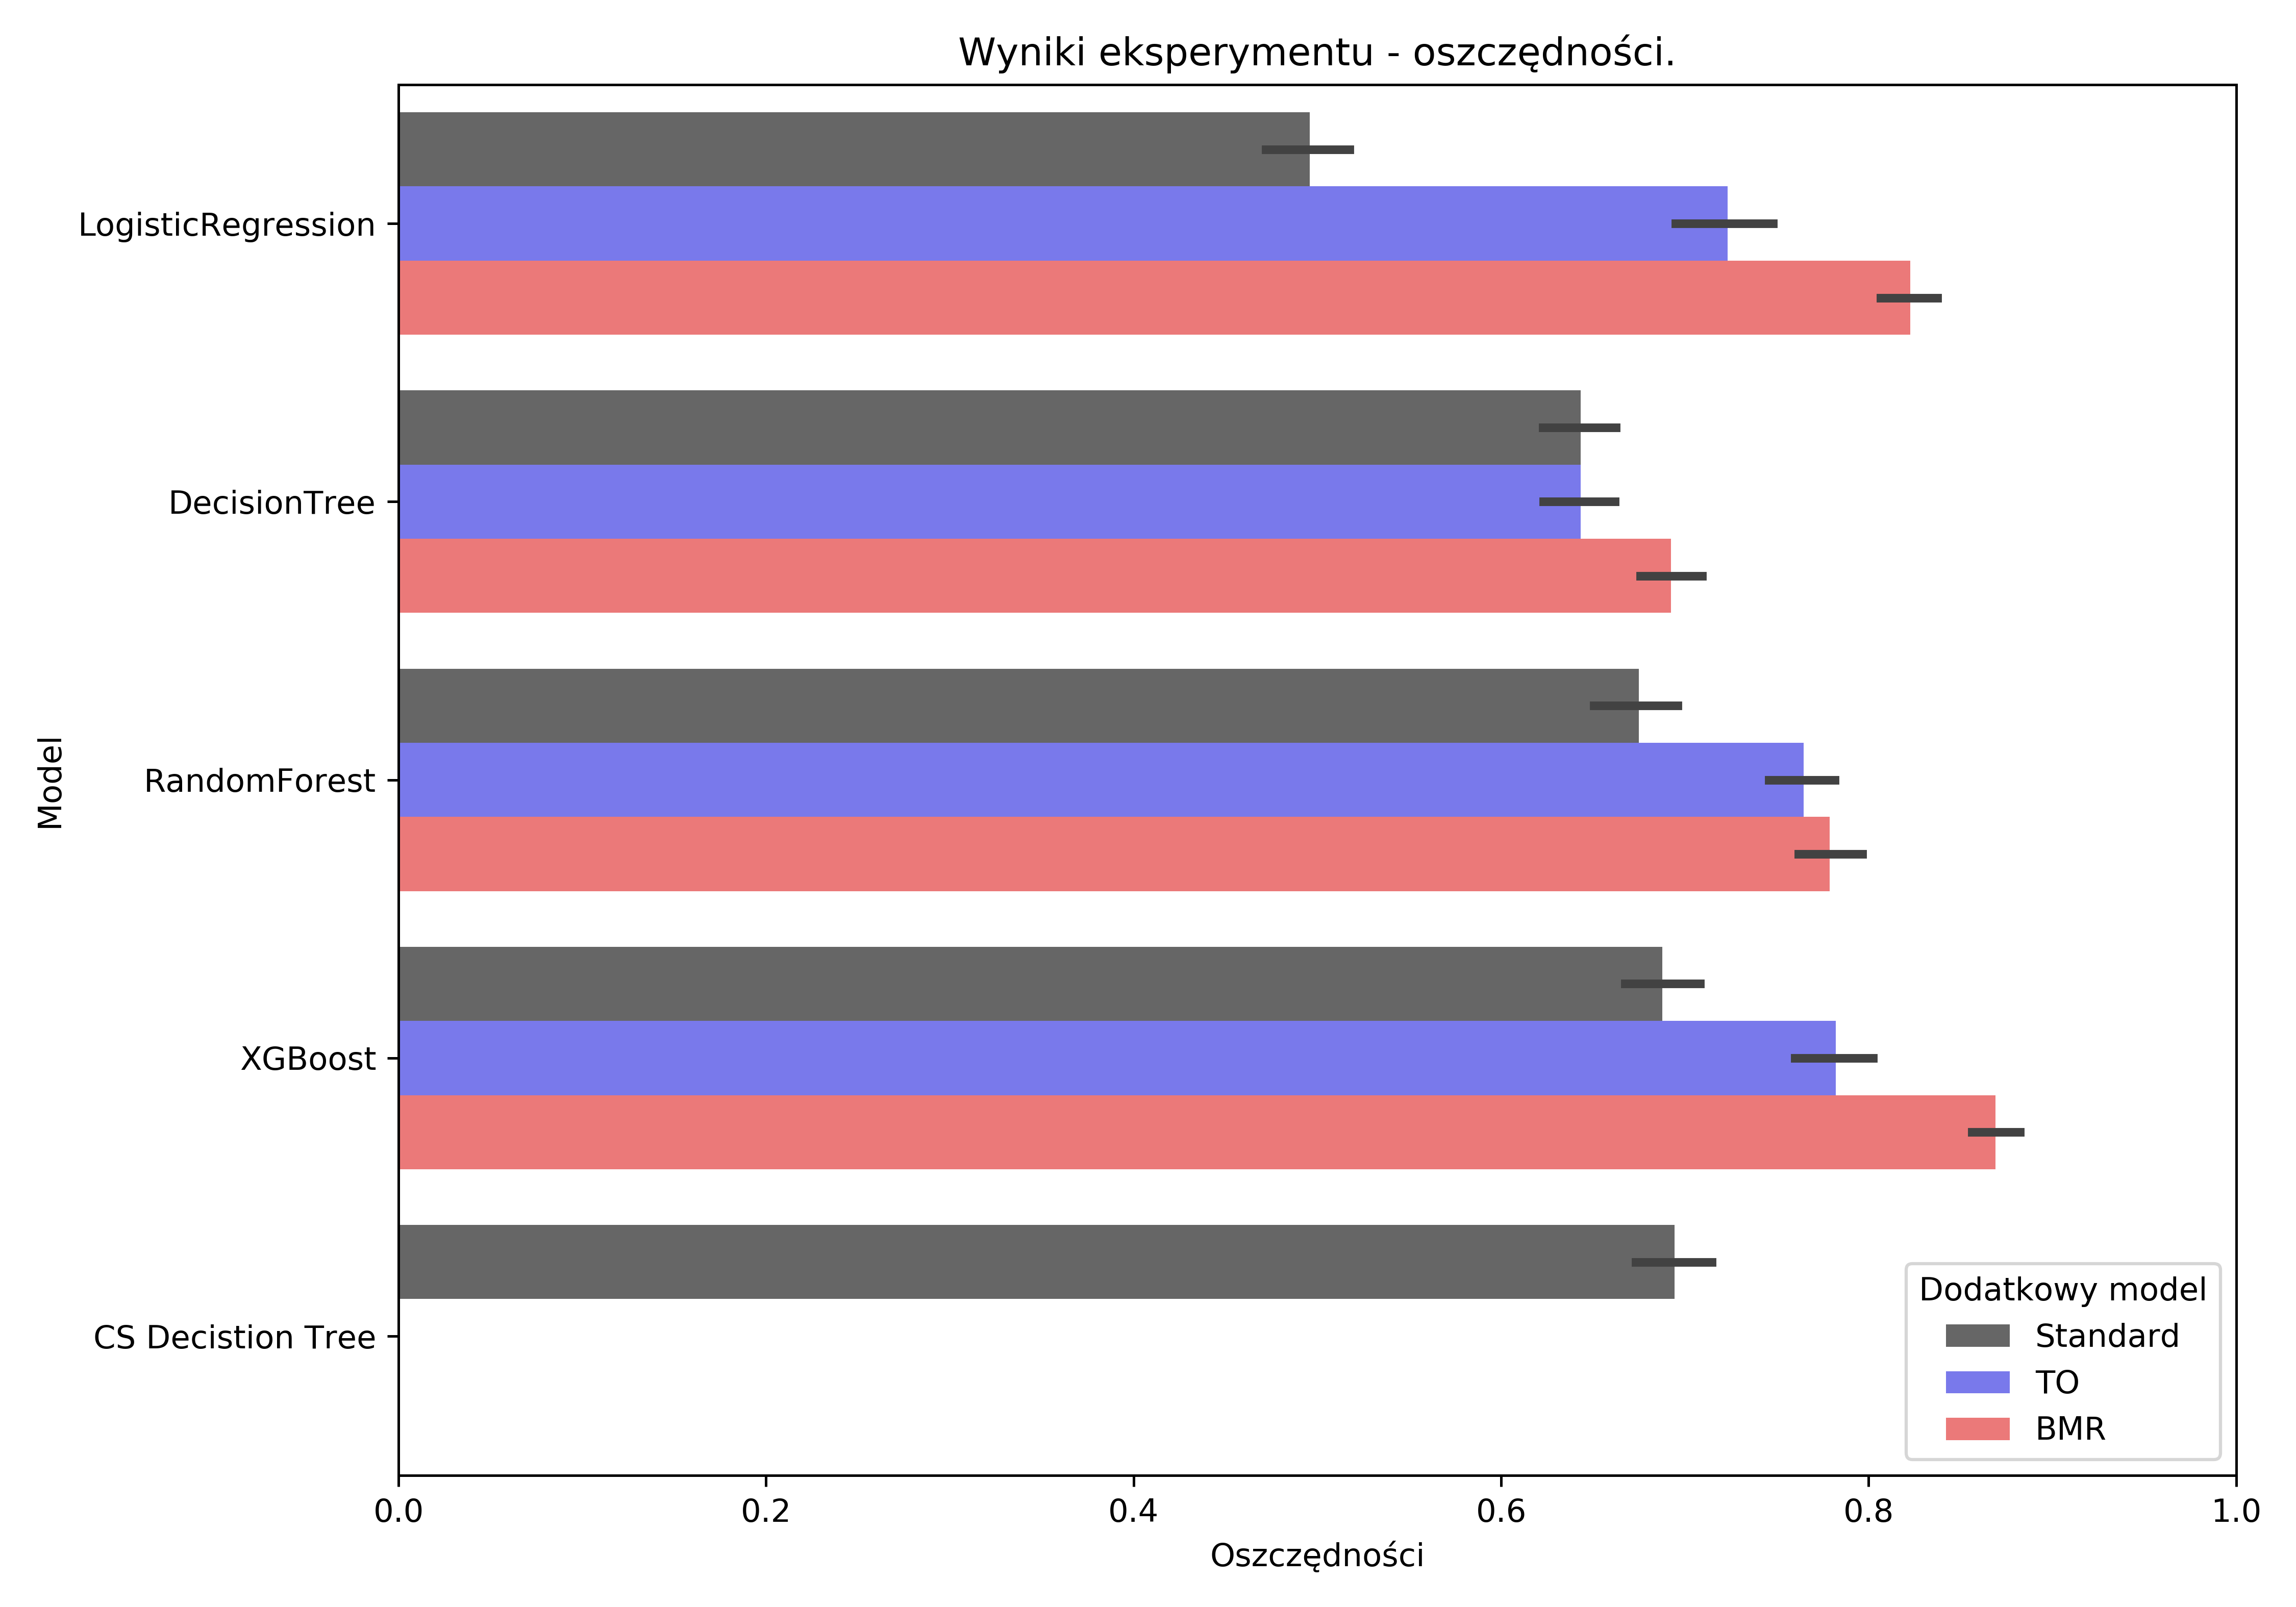
\includegraphics[width=\linewidth]{images/100_config1-Savings.png}
	\caption{Wyniki eksperymentu dla miary skuteczności oszczędności. Szare, niebieskie oraz czerwone słupki oznaczają dla pierwszych czterych modeli: regresji logistycznej (LogisticRegression), drzewa decyzyjnego (DecisionTree), lasu losowego (RandomForest) oraz XGBoosta, odpowiednio model standardowy, model optymalziacji progu oraz model wykorzystujący minimalizację ryzyka bayesowskiego. Dla modelu drzewa decyzyjnego wrażliwego na koszt (CS Decision Tree) szary słupek oznacza wynik dla modelu wrażliwego na koszt. Wysokość słupka reprezentuje wartość średnią z 50 powtórzeń, a długość dołączonej kreski oznacza $\pm$ wartość odchylenia standardowego w odpowiednią stronę. Źródło: Opracowanie własne.}
	\label{fig:results-savings}
\end{figure}

W tym celu przeanalizujemy wyniki eksperymentu dla miary skuteczności $F_1$ Score, które są zaprezentowane na wykresie \ref{fig:results-f1} na stronie \pageref{fig:results-savings}. Oznaczenia są analogiczne do wykresu dotyczącego oszczędności. Możemy zauważyć, że dla standardowych wersji modeli w przypadku tej miary skuteczności najlepsze rezultaty osiągnął las losowy oraz XGBoost. Dodatkowo model drzewa decyzyjnego wrażliwego na koszt uzyskał w~tym wypadku gorsze rezultaty niż standradowa wersja. W~przypadku klasyfikacji wrażliwej na koszt modele optymalizacji progu prawie zawsze pogarszały wyniki (z wyjątkiem drzewa decyzjnego, gdzie wynik był taki sam jak bez modelu), a dla minimalizacji ryzyka bayesowskiego wynik zawsze był gorszy od standardowej wersji modelu. Intuicyjnie jest to zrozumiały rezultat, ponieważ nasz model przestał zwracać uwagę na transakcje, który miały małą wartość, nawet jeżeli przypadek ten był łatwy do wykrycia, a profilaktycznie zaczął sprawdzać duże transakcje, które mogły mieć nawet małe prawdopodobieństwa bycia oszustwem. W związku z tym modele zaczęły oszczędzać więcej pieniędzy kosztem ogólnej skuteczności modelu i zwracaniem większej ilości fałszywie pozytywnych klasyfikacji. 

\begin{figure}[h]
	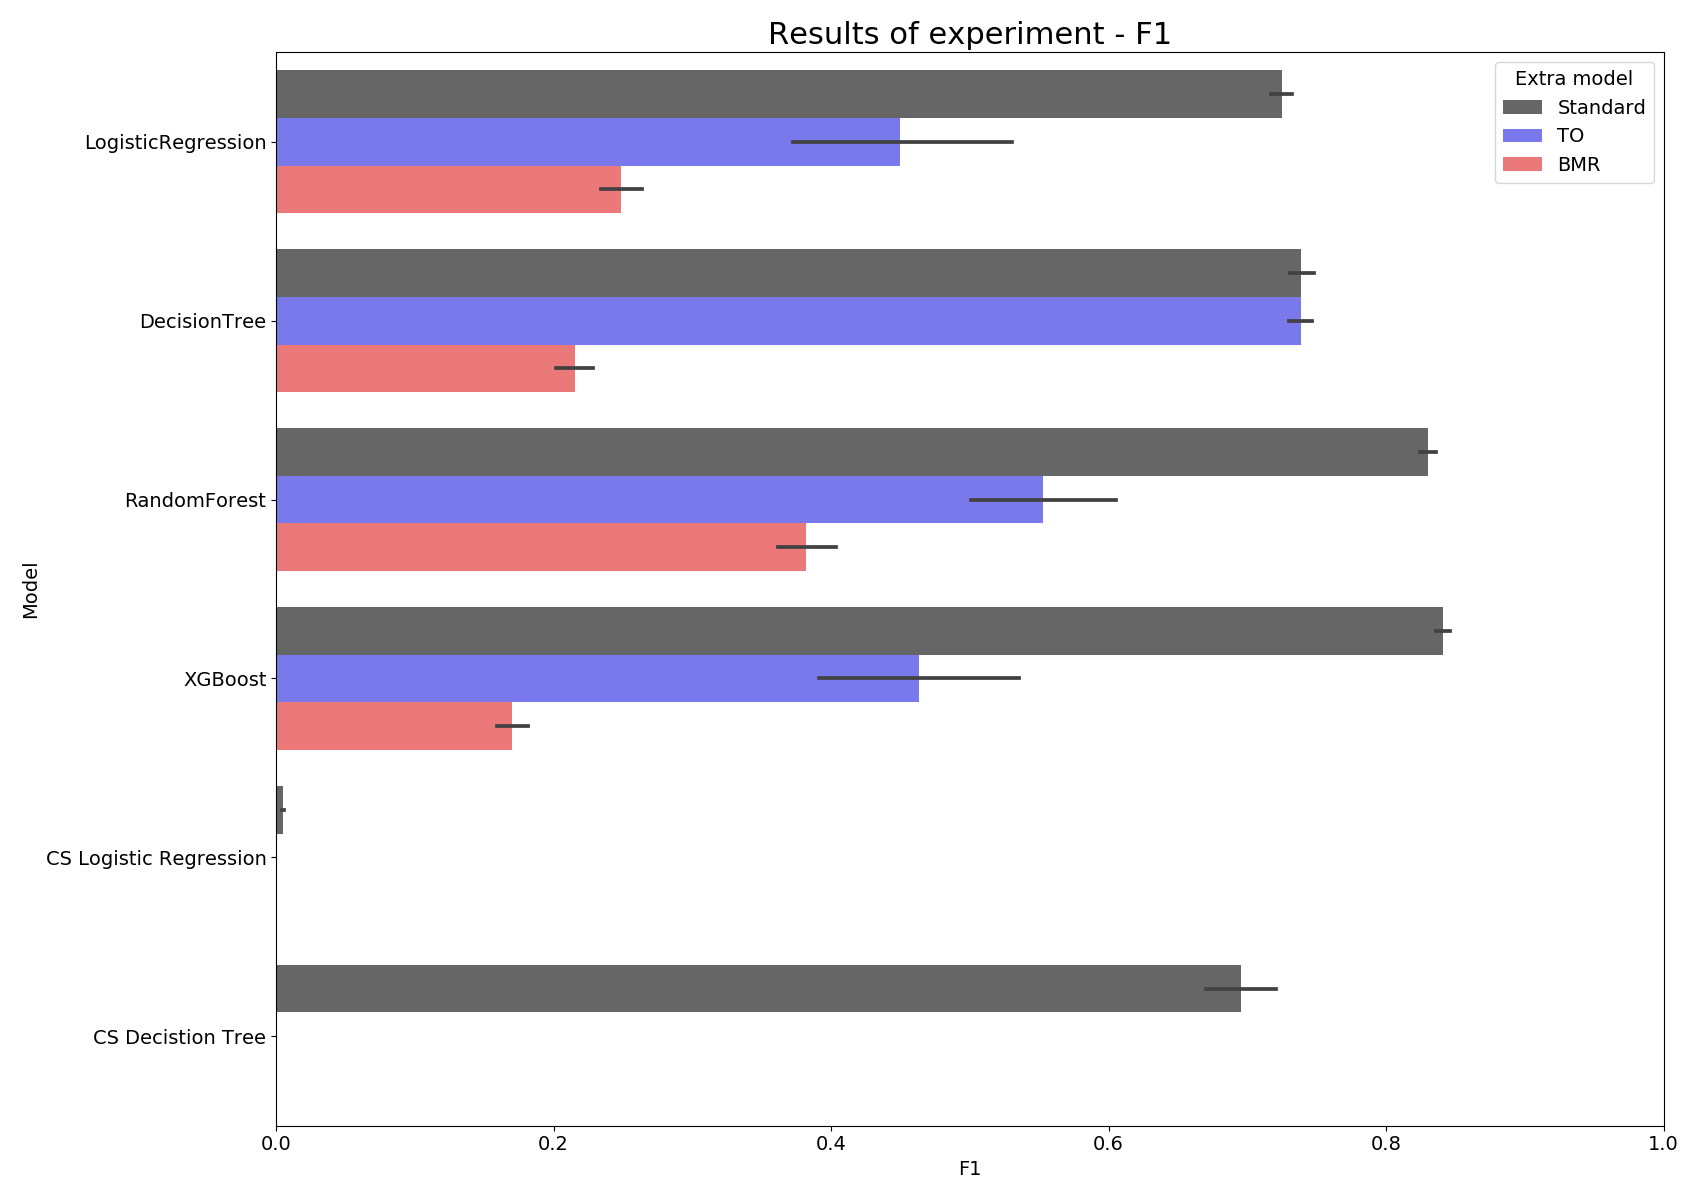
\includegraphics[width=\linewidth]{images/100_config1-F1.png}
	\caption{Wyniki eksperymentu dla miary skuteczności F1-Score. Szare, niebieskie oraz czerwone słupki oznaczają dla pierwszych czterych modeli: regresji logistycznej (LogisticRegression), drzewa decyzyjnego (DecisionTree), lasu losowego (RandomForest) oraz XGBoosta, odpowiednio model standardowy, model optymalziacji progu oraz model wykorzystujący minimalizację ryzyka bayesowskiego. Dla modelu drzewa decyzyjnego wrażliwego na koszt (CS Decision Tree) szary słupek oznacza wynik dla modelu wrażliwego na koszt. Wysokość słupka reprezentuje wartość średnią z 50 powtórzeń, a długość dołączonej kreski oznacza $\pm$ wartość odchylenia standardowego w odpowiednią stronę. Źródło: Opracowanie własne.}
	\label{fig:results-f1}
\end{figure}

Zestawiając uzyskane rezultaty z obu miar, możemy dojść do wniosku, że jeżeli najważniejszym i jedynym kryterium, które chcemy rozważać w ocenie jakości modelu, są oszczędności, to w przypadku tego zbioru danych najlepszym wyborem jest algorytm XGBoost z minimalizacją ryzyka bayesowskiego. Natomiast jeżeli poza oszczędnościami chcemy wziąć także pod uwagę ogólną jakość predykcyjną modelu, to wyniki nie jest aż tak jednoznaczny i w~zależności od przypadku będziemy musieli wybierać pomiędzy ogólną skuteczność a oszczędnościami. Ciekawym wyborem w~tym przypadku może być drzewo decyzyjne wrażliwe na koszt, las losowy lub XGBoost w wersji standardowej. Dodatkową informacją, która mogłaby nam pomóc podjąć decyzję, może być ilość pozytywnych przypadków z każdego modelu oraz ilość analityków zajmujących się sprawdzaniem oszustw, ponieważ może się okazać, że w wyniku zbyt małej ilości osób nie będziemy w stanie sprawdzić wszystkich wytypowanych spraw. W~takiej sytuacji model, który typuje mniej transakcji do sprawdzania przy zachowaniu podobnych skuteczności obu miar, może okazać się najlepszym wyborem. Z~drugiej strony, jeżeli taka informacja byłaby dostępna na początku modelowania, to wymusiłaby ona dodatkowe założenia i podejście do procesu doboru metryk.

\chapter*{Podsumowanie}
Pracę rozpoczęliśmy od wprowadzenia problemu detekcji oszustw na kartach kredytowych oraz omówienia aktualnego podejścia do tworzenia systemów wykrywających oszustwa. Następnie omówiliśmy rodzaje miar, które są standardowo wykorzystywane w statystyce oraz uczeniu maszynowym, a także miary, które stosuje się w~problemach wrażliwych na koszt. Dalej opisaliśmy podstawy teoretyczne standardowych modeli predykcyjnych, ich modyfikacji wrażliwych na koszt oraz klasyfikatorów wrażliwych na koszt. W~ostatniej części pracy przeprowadziliśmy eksperyment, którego celem było porównanie wybranych klasyfikatorów na danych rzeczywistych dotyczących detekcji oszustw na kartach kredytowych.

Na podstawie przeprowadzonego eksperymentu ustaliliśmy, że na tym konkretnym zbiorze danych dzięki wykorzystaniu metod wrażliwych na koszt bylibyśmy w stanie zwiększyć oszczędności w problemie detekcji oszustw na kartach kredytowych. Najlepszym modelem pod tym względem okazał się XGBoost, który do tej pory nie był rozważanych w pracach A.~Bahnsena dotyczących podobnych zagadnień. Dodatkowo zauważyliśmy, że wykorzystanie klasyfikatorów wrażliwych na koszt znacząco obniża skuteczność modelu w~sensie standardowych miar. W~przypadku, gdybyśmy chcieli zachować balans pomiędzy tymi dwoma miarami, najlepszych wyborem byłby algorytm XGBoost, las losowy lub drzewo decyzyjne wrażliwe na koszt.

Na podstawie przeprowadzonych badań wydaje się, że bardzo ciekawym kierunkiem do dalszych rozważań mogą być metody typu \textit{ensemble}, których klasyfikatorem bazowym byłoby drzewo decyzyjne wrażliwe na koszt. Takie działania zostały już podjęte dla lasów losowych w cytowanej wcześniej pracy A.~Bahnsena \cite{alej2015ensemble}. Z uwagi na fakt, że algorytm XGBoost otrzymywał najlepsze rezultaty dla obu miar skuteczności oraz drzewo decyzyjne w wersji wrażliwej na koszt uzyskiwało lepsze rezultaty niż standradowa wersja modelu, daje to nadzieje, że XGBoost wrażliwy na koszt może dawać jeszcze lepsze wyniki.

% Bibliografia
\backmatter
\nocite{*}

\bibliografia{references} 

\end{document}